\documentclass[10pt, letterpaper]{report}
\input{../University_notes/preamble/preamble.tex}
\title{Geometria Differenziale}
\author{Marco Casu}
\date{\vspace{-5ex}}
\begin{document}
\definecolor{bluchiaro}{HTML}{9fb0cf}
\newpage
\pagecolor{cartaRiciclata}
\color{black}
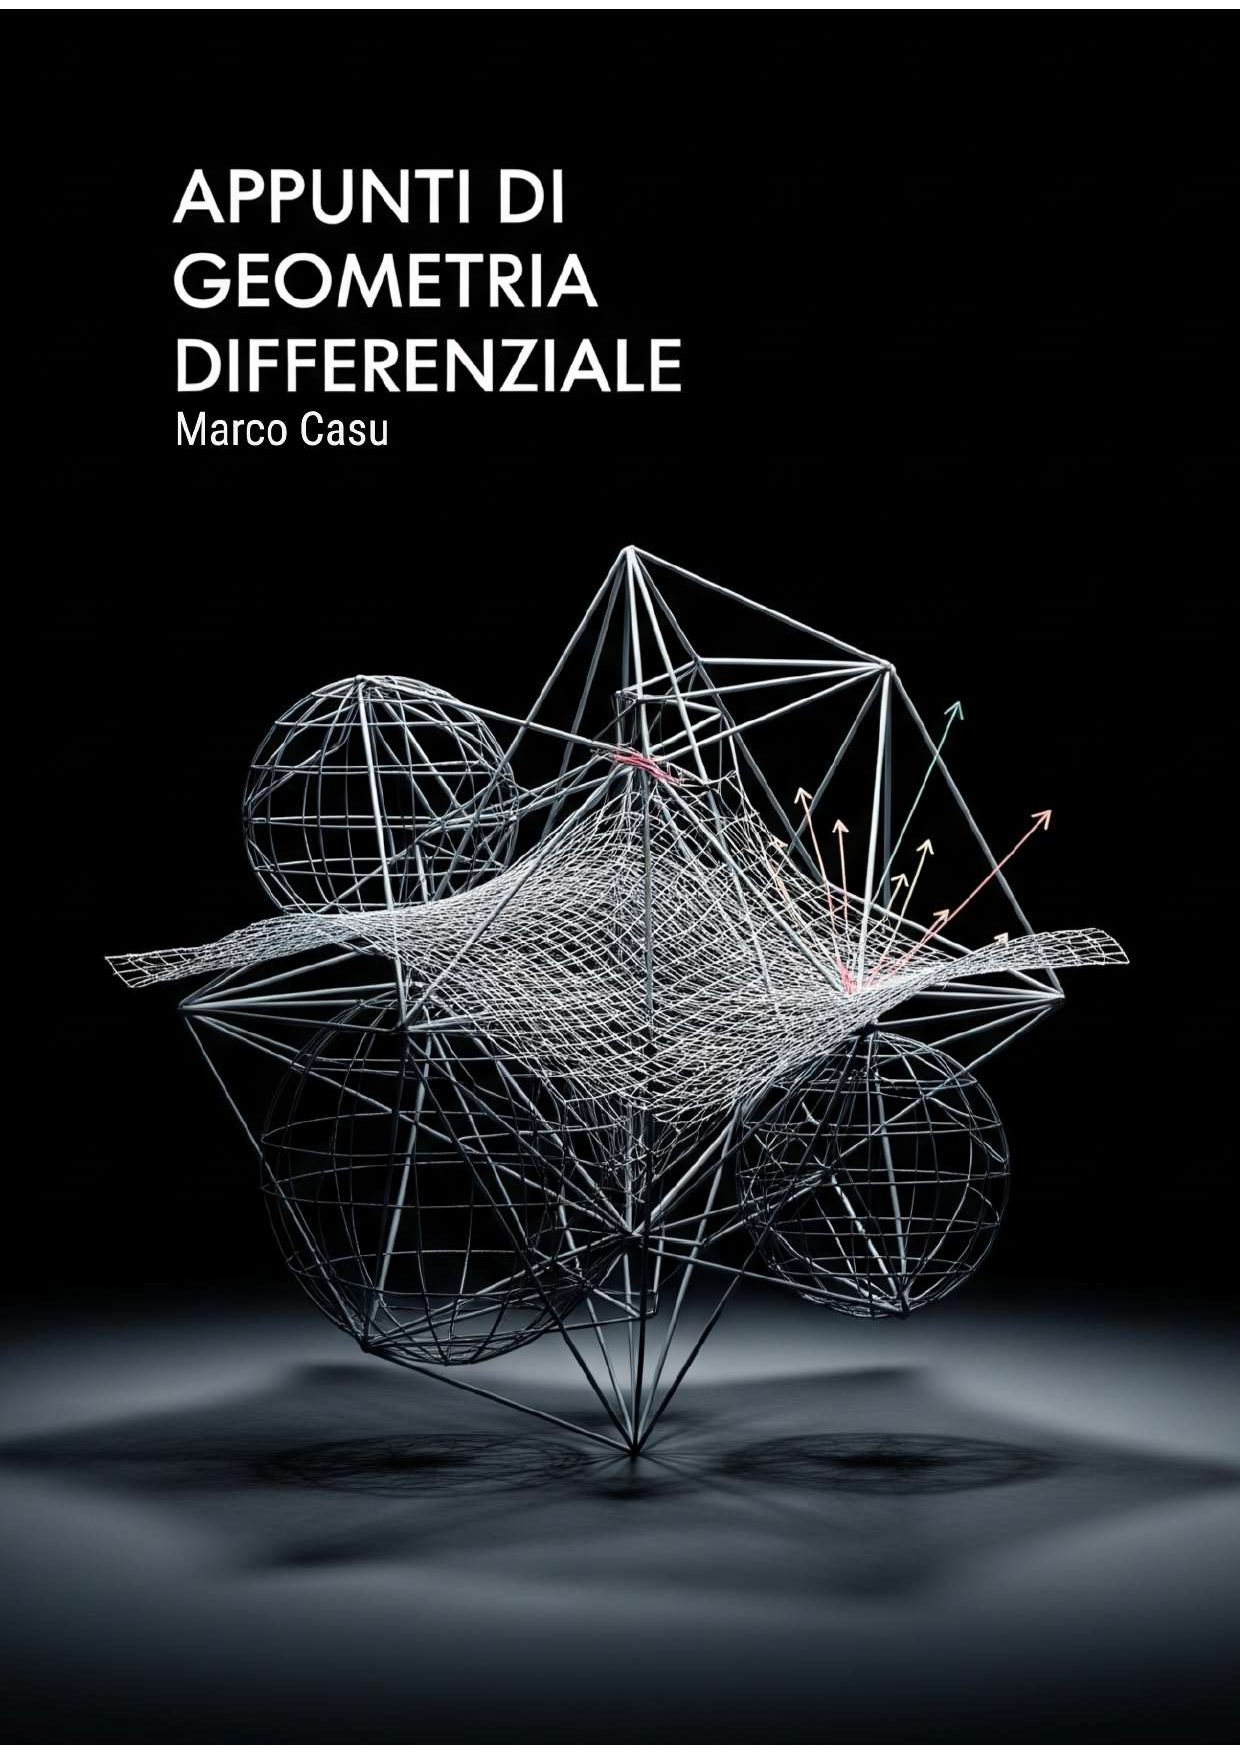
\includepdf{images/copertina.pdf}
\noindent I seguenti appunti sono tratti dal corso di Geometria Differenziale tenuto dal docente Francesco Bottacin per l'Università degli Studi di Padova.
\tableofcontents \newpage

\fancyhf{}
\fancyhead[L]{\nouppercase{\leftmark}}
\fancyhead[R]{Sezione \thesection}
\fancyfoot[C]{\thepage}
\fancyfoot[L]{Geometria Differenziale}
\fancyfoot[R]{Marco Casu}
\newtheorem{definizione}{Definizione}
\newtheorem{teorema}{Teorema}
\newtheorem{esercizio}{Esercizio}
\newtheorem{congettura}{Congettura}
\newtheorem{lemma2}{Lemma}
\newtheorem{proposizione}{Proposizione}
\newtheorem{osservazione}{Osservazione}


\chapter{Varietà Differenziabili}
\section{Definizioni Preliminari, Varietà Topologiche}
Uno degli scopi della geometria differenziale è quello di ricondurro lo studio di oggetti di forme complicate allo studio di un certo sotto-insieme di $\R^n$, si consideri una superficie sferica in $\R^3$
\begin{equation}
    S^{2}=\{\mathbf x\in\R^3 \ : \ \|\mathbf x\|_2=1\}
\end{equation}
denotando con $\|\cdot\|_2$ la norma euclidea. Ogni punto della sfera (esclusi i poli) può essere individuato da due coordinate reali $(\varphi,\theta)\in[-\frac{\pi}{2},\frac{\pi}{2}]\times[0,2\pi]\subset\R^2$, dette latitudine e longitudine, come mostrato in figura \ref{img:sfera}. Si è introdotto un'opportuno sistema di coordinate allo scopo di ricondurre lo studio della sfera allo studio di un sottoinsieme di $\R^2$.
\begin{figure}[h!]
    \center
    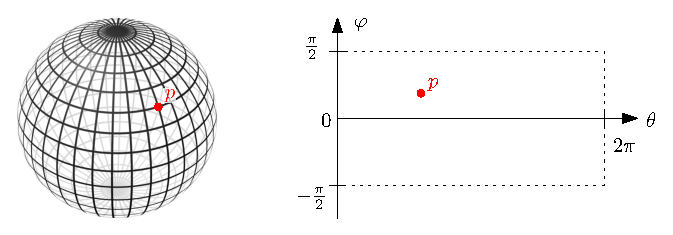
\includegraphics[width=0.8\textwidth ]{images/sfera.eps}
    \caption{Sistema di coordinate per la sfera in $\R^3$}
    \label{img:sfera}
\end{figure}
\begin{definizione}
Sia $X$ un'insieme, e $\tau$ una collezione di sottoinsiemi di $X$, $\tau$ è una \textbf{topologia} in $X$ se\begin{itemize}
    \item $\emptyset\in\tau$ e $X\in\tau$
    \item Se $V_i\in\tau$ per $i=1,2\dots,n$ allora $\displaystyle\bigcap_{1\le i\le n}
    V_i\in\tau$
    \item Se $\{V_{\alpha}\}$ è una collezione di elementi di $\tau$ (finita, numerabile o non numerabile) allora $\displaystyle\bigcup_{\alpha}V_i\in\tau$.
\end{itemize}
\end{definizione}
\begin{definizione}
    Se un'insieme $X$ ammette una topologia $\tau$ allora $X$ è uno \textbf{spazio topologico} e gli insiemi in $\tau$ si dicono \textbf{insiemi aperti} di $X$.
\end{definizione}
\begin{definizione}
    Se $X$ e $Y$ sono due spazi topologici, una funzione $f:X\rightarrow Y$ è \textbf{continua} se, per ogni aperto $V$ di $Y$, l'insieme $f^{-1}(V)$ è un'aperto di $X$.
\end{definizione}
\begin{definizione}
    Una funzione $f:X\rightarrow Y$ fra due spazi topologici è un \textbf{omeomorfismo} se è biettiva, continua, e la sua inversa $f^{-1}$ è anch'essa continua.
\end{definizione}
$\R^n$ è il più semplice esempio di spazio topologico.
La seguente definizione è fondamentale e necessaria alla successiva definizione di \textit{varietà}.
\begin{definizione}
    Sia $X$ uno spazio topologico e $U\subset X$ un'aperto, sia $\varphi$ un \textit{omeomorfismo} da $U$ ad un aperto di $\R^n$\begin{eqnarray}
        \varphi:U\rightarrow\varphi(U)\subset \R^n\\ 
        \varphi(U) \text{ è un'insieme aperto}
    \end{eqnarray}
    allora la coppia $(U,\varphi)$ è una \textbf{carta} per $X$.
\end{definizione}
\begin{figure}[h!]
    \center
    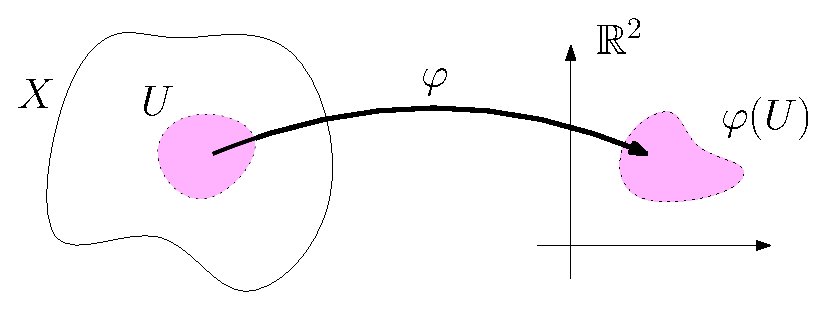
\includegraphics[width=0.55\textwidth ]{images/carta.eps}
    \caption{Una carta da un'insieme $X$ ad un'aperto di $\R^2$}
    \label{img:carta}
\end{figure}
In tal contesto la funzione inversa $\varphi^{-1}$ è detta \textit{parametrizzazione locale}. Si considera ora il caso in cui due carte si intersecano, ossia, per uno stesso spazio topologico $X$, vi sono due carte $(U_1,\varphi_1),(U_2,\varphi_2)$ tali per cui $U_1\cap U_2\ne\emptyset$, come mostrato in figura \ref{img:intersezione_carte}.
\begin{figure}[h!]
    \center
    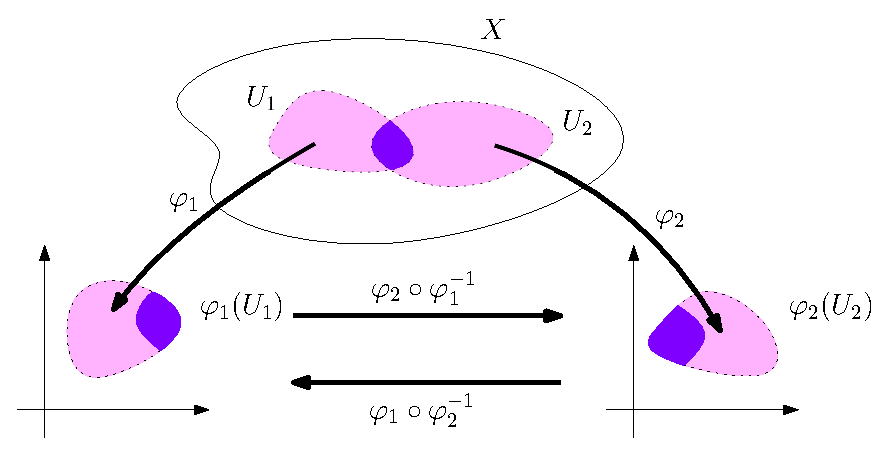
\includegraphics[width=0.7\textwidth ]{images/intersezione_carte.eps}
    \caption{Intersezione fra due carte in $X$}
    \label{img:intersezione_carte}
\end{figure}

La funzione $\varphi_2\circ\varphi_1^{-1}$ è definita solamente sulla regione $\varphi_1(U_1\cap U_2)\subset\R^n$, mentre $\varphi_1\circ\varphi_2^{-1}$ è definita solamente sulla regione $\varphi_2(U_1\cap U_2)\subset\R^n$, si ometterà tale restrizione nella notazione, e si assumerà che tali funzioni sono definite esclusivamente sugli insiemi menzionati.\bigskip

\noindent 
Le funzioni $\varphi_2\circ\varphi_1^{-1}$,$\varphi_1\circ\varphi_2^{-1}$ sono omeomorfismi tra aperti di $\R^n$. Da questo punto in avanti, date due carte $(U_i,\varphi_i),(U_j,\varphi_j)$, si denoterà\begin{equation}
    \eta_{ij}=\varphi_i\circ\varphi_j^{-1}
\end{equation}
queste sono denominate \textbf{funzioni di transizione} e descrivono il cambiamento di coordinate fra due differenti aperti di $\R^n$. Le funzioni di transizione definiscono la relazione fra punti che si trovano su più insiemi aperti di $X$ sui quali sono definite differenti carte. Le funzioni di transizione soddisfano le seguenti identità:\begin{itemize}
    \item $\eta_{ii}=\text{Id}$
    \item $\eta_{ij}=\eta_{ji}^{-1}$
    \item su $U_i\cap U_j\cap U_k$ si ha $\eta_{ij}\circ\eta_{jk}=\eta_{ik}$.
\end{itemize}
\begin{definizione}
    Sia $X$ uno spazio topologico, e sia $\{(U_i,\varphi_i)\}_{i\in I}$ una famiglia di carte tali per cui \begin{equation}
         X=\bigcup_{i\in I}U_i
    \end{equation}
    in tal caso l'insieme $\{(U_i,\varphi_i)\}_{i\in I}$ è un \textbf{atlante} per $X$.
\end{definizione}
\begin{definizione}
     Sia $X$ uno spazio topologico, se esiste un atlante per $X$, quest'ultima è detta \textbf{varietà topologica}.
\end{definizione}
\begin{definizione}
    Uno spazio topologico si dice \textbf{connesso} se non può essere rappresentato come l'unione di due o più insiemi aperti non vuoti e disgiunti.
\end{definizione}
Da questo punto in avanti si assumerà che gli spazi topologici considerati siano connessi.
Un'atlante per uno spazio topologico $X$ è una famiglia di carte che ricopre l'intero spazio, si considerino due differenti carte su $X$ tali per cui 
\begin{align}
    &\varphi_1:U_1\rightarrow\varphi_1(U_1)\subset \R^n\\ 
    &\varphi_2:U_2\rightarrow\varphi_2(U_2)\subset \R^m
\end{align}
se $U_1\cap U_2\ne \emptyset$ la funzione di transizione $\eta_{12}$ è un omeomorfismo tra un'aperto di $\R^m$ ad un'aperto di $\R^n$, necessariamente $n=m$ (la dimostrazione è omessa).
\begin{osservazione}
Se $X$ è una varietà topologica connessa, tutte le carte di un'atlante per $X$ sono funzioni che hanno come ambiente per il codominio $\R^n$, con $n$ fissato in comune per ogni carta, in tal caso si dice che $n$ è la \textbf{dimensione} della varietà $X$.
\end{osservazione}
La dimensione di una varietà è quindi ben definita dalle carte locali.
\section{Funzioni Differenziabili sulle Varietà}
Sia $X$ una varietà topologica di dimensione $n$, con atlante $\{(U_i,\varphi_i)\}$. Si consideri una funzione continua $f:X\rightarrow\R$, si ha:
\[
\begin{tikzcd}
X \supset U_i \arrow[r, "{\varphi}_i"] \arrow[d, "f_{|U_i}"'] & \varphi(U_i) \subset \mathbb{R}^n \arrow[dl, "\tilde{f}_i"] \\
\mathbb{R} &
\end{tikzcd}
\]
ove $\tilde{f}_i=f_{|U_i}\circ\varphi_i^{-1}$. La funzione $\tilde{f}_i:\varphi(U_i)\rightarrow \R$ è una funzione definita su un'aperto di $\R^n$, sui quali si possono adoperare i metodi di studio dell'Analisi. 
Se $U_i\cap U_j\ne\emptyset$, allora la funzione $\tilde f_j:\varphi(U_j)\rightarrow \R$ si può riscrivere $\tilde f_j=\tilde f_i\circ \eta_{ij}$\begin{itemize}
    \item $\eta_{ij}$ è un omeomorfismo da un'aperto di $\R^n$ ad'un aperto di $\R^n$
    \item $\tilde f_i$ è una funzione da un'aperto di $\R^n$ ad'un'aperto di $\R$
    \item $\tilde f_j=\tilde f_i\circ \eta_{ij}$ è una funzione da un'aperto di $\R^n$ ad'un'aperto di $\R$.
\end{itemize}
Un diagramma commutativo è dato in figura \ref{img:intersezione_carte_fun}.
\begin{figure}[h!]
    \center
    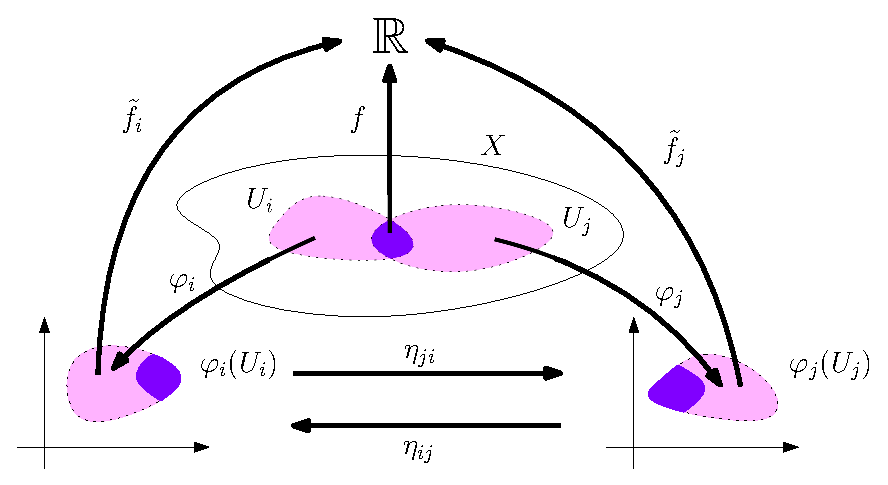
\includegraphics[width=0.7\textwidth ]{images/intersezione_carte_func.eps}
    \caption{La funzione $f$ in relazione con l'intersezione fra due carte in $X$}
    \label{img:intersezione_carte_fun}
\end{figure}
$\tilde f_i$ è la rappresentazione locale della funzione $f$ sull'aperto $U_i\subset X$. $\tilde f_i$ e $\tilde f_j$ sono funzioni differenti che rappresentano però la stessa funzione $f$, ma in sistemi di coordinate differenti.

Se si vuole descrivere una funzione $f$ definita in $X$, si può definire localmente tramite un'atlante su $X$, ove per ciascuna carta locale $\varphi_i$ si identifica l'espressione locale di $f$, denotata $\tilde f_i$, vi è una funzione di questo tipo per ogni carta dell'atlante. Le funzioni $\tilde f_i$ sono descrizioni di $f$, non possono essere funzioni scelte arbitrariamente, ma devono soddisfare la relazione \begin{equation}
    \tilde f_j = \tilde f_i\circ\eta_{ij}
\end{equation}
per ogni funzione di transizione $\eta_{ij}$.\begin{osservazione}
    Usando tale fatto, si è ricondotto il problema di studiare una funzione $f$ su una varietà topologica, al problema dello studio di funzioni $\tilde f_i$ definite su aperti di $\R^n$.
\end{osservazione}
Si vuole definire ora la \textit{differenziabilità} di $f$ definita su una varietà topologica. Una funzione è di classe $C^r$ definita su $U$ aperto di $\R^n$ se tutte le sue derivate parziali fino all'ordine $r$ esistono e sono continue su $U$. Potremmo dire che $f$ definita su una varietà topologica $X$ è di classe $C^r$ su $U_i$ aperto di $X$ se e solo se una sua rappresentazione locale $\tilde f_i$ è di classe $C^r$ in $\varphi(U_i)$, ma ciò è errato in quanto si deve considerare il fatto che possa esistere una differente carta $(U_j,\varphi_j)$ che si interseca con $U_i$, tale per cui $\tilde f_j$ è di classe $C^{r'}$ con $r'<r$.
\begin{definizione}
    Una varietà topologica $X$ è di classe $C^r$ se tutte le funzioni di transizione $\eta_{ij}$ sono di classe $C^s$ con $s\ge r$.
\end{definizione}
\begin{osservazione}
    Se una varietà $X$ è di classe $C^s$, si può definire la nozione di funzione $f$ di classe $C^r$ su $X$, con $r\le s$.
\end{osservazione}
\begin{definizione}
    Una varietà topologica di classe $C^\infty$ è detta \textbf{varietà differenziabile}. Se $n$ è la dimensione della varietà, si denominerà semplicemente $n$-varietà.
\end{definizione}
Sulle funzioni definite su una varietà differenziabile si possono applicare i metodi del calcolo differenziale propri dell'Analisi. Essendo che ogni punto di una varietà $X$ è contenuto in un'intorno aperto omeomorfo ad un'insieme aperto di $\R^n$, le proprietà locali di una varietà sono le stesse della topologia in $\R^n$, in particolare ogni varietà è:\begin{itemize}
    \item \textit{localmente compatta}
    \item \textit{localmente connessa}
\end{itemize}
per completezza, saranno date le definizioni di tali proprietà.
\begin{definizione}
    Uno spazio topologico $X$ si dice \textbf{compatto} se da ogni suo ricoprimento costituito da una famiglia di insiemi aperti si può estrarre una sottofamiglia finita che è ancora un ricoprimento. Sia $\{U_i\}_{i\in I}$ una qualsiasi famiglia di sottoinsiemi aperti di $X$ tali per cui\begin{equation}
        \bigcup_{i\in I}U_i=X 
    \end{equation}
    allora esiste un sottoinsieme finito $J\subset I$ tale per cui
    \begin{equation}
        \bigcup_{i\in J}U_i=X .
    \end{equation}
\end{definizione}
\begin{definizione}
    uno spazio topologico $X$ è detto \textbf{localmente compatto} se per ogni suo punto esiste un intorno la cui chiusura è un insieme compatto. Si ricordi che la chiusura di un'aperto $U$ è l'intersezione di tutti gli insiemi chiusi contenenti $U$.
\end{definizione}
\begin{definizione}
    Uno spazio topologico $X$ è \textbf{localmente connesso} se ogni punto dello spazio ha un sistema di intorni connessi. Si ricordi che un sistema di intorni è un insieme di intorni tale che qualsiasi intorno aperto di $x\in X$ contiene uno di questi intorni.
\end{definizione}
Si assumerà (solitamente) che ogni varietà differenziabile $X$ considerata sia uno spazio topologico di Hausdorff, ossia per il quale vale il seguente assioma:\begin{equation}
    \forall x,y\in X\ : \ x\ne y \ \exists U,V \text{ intorni aperti di }x,y\text{ tali che }U\cap V = \emptyset .
\end{equation}
\subsection{Esempi di Varietà}
Sono dati in seguito alcuni esempi di varietà differenziabili.\bigskip


\noindent\textbf{Esempio 1} $\R^n$ è una varietà differenziabile, anche ogni aperto di $\R^n$ lo è. Un qualunque spazio vettoriale reale di dimensione finita è isomorfo a $\R^n$, è quindi anch'esso una varietà.
\begin{osservazione}
    Anche uno spazio vettoriale a dimensione infinita può essere una varietà differenziabile, è però necessario considerare una definizione alternativa di carta, in cui non si esclude il fatto che l'immagine di una carta locale possa essere uno spazio vettoriale di dimensione infinita.
\end{osservazione}
\textbf{Esempio 2} Se $X$ è una varietà e $U\subset X$ è un'insieme aperto, allora $U$ è una varietà.
\bigskip

\noindent\textbf{Esempio 3} Il prodotto di due varietà è una varietà. Si consideri una $m$-varietà $X$ ed una $n$-varietà $Y$, sia $\mathcal A$ un'atlante per $X$ e $\mathcal B$ un'atlante per $Y$\begin{align}
    &\mathcal A = \{(U_\alpha,\varphi_\alpha)\}\\
    &\mathcal B = \{(V_\beta,\psi_\beta)\}.
\end{align}
Sia $\mathcal A\times \mathcal B=\{(U_\alpha\times V_\beta,\varphi_\alpha\times \psi_\beta)\}$ ove\begin{align}
    &\varphi_\alpha\times\psi_\beta:U_\alpha\times V_\beta\rightarrow\R^m\times \R^n=R^{m+n}\\ &
    (x,y)\longmapsto (\varphi_\alpha(x),\psi_\beta(y)).
\end{align}
Questo è un atlante per $X\times Y$, quest'ultima è quindi una $n+m$-varietà.
\bigskip

\noindent\textbf{Esempio 4} Si consideri l'insieme \begin{equation}
    GL(n,\R)=\{A\in M(n,\R) \ : \ \det A\ne 0\}
\end{equation}
ossia l'insieme delle matrici quadrate $n\times n$ a valori reali il cui determinante è diverso da zero, questo è un sottoinsieme aperto di $\R^{n^2}$, quindi è una varietà. Il fatto che sia aperto è dato dal fatto che l'insieme delle matrici con determinante nullo è un'insieme chiuso.
\bigskip

\noindent\textbf{Esempio 5} Si consideri la sfera $S_R^{n}$ di raggio $R$ in $\R^{n+1}$
\begin{equation}
    S^{n}_R=\{\mathbf x\in\R^{n+1} \ : \ \|\mathbf x\|_2=R\}
\end{equation}
è uno spazio topologico la cui topologia è quella indotta di $\R^{n+1}$. Si definirà un'atlante per $S_R^{n}$ costituito da due carte.
Si considerino i due poli\begin{align}
    &N=(0,0,0\dots,R)\\
    &S=(0,0,0\dots,-R)
\end{align}
si denota $p=(p^1,\dots,p^{n+1})$ un generico punto della sfera, si noti come le coordinate si identificano con degli apici piuttosto che con dei pedici, l'utilità di tale notazione sarà chiarita in seguito.
    
Sia $\pi$ l'iperpiano di equazione $x^{n+1}=0$, naturalmente identificato con $\R^n$. La prima carta è $(S_R^{n}\backslash\{N\},\varphi_N)$ \begin{equation}
    \varphi_N:S_R^{n}\backslash\{N\}\rightarrow\pi\simeq\R^n
\end{equation}
definita come la \textit{proiezione stereografica}. Il punto $\varphi_N(p)\in\R^n$ identificato, è il punto che si trova su $\pi$ attraversato dall'unica retta che passa per $p$ e per $N$. Un'esempio in $\R^3$ è riportato in figura \ref{img:proiezione_stereografica}.

\begin{figure}[h!]
    \center
    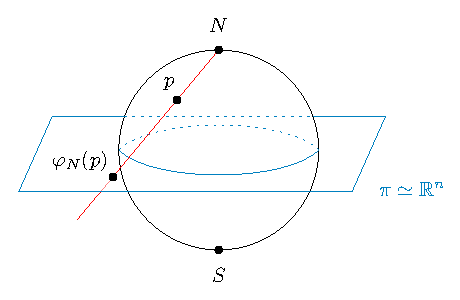
\includegraphics[width=0.4\textwidth ]{images/proiezione_stereografica.eps}
    \caption{Proiezione stereografica in $\R^3$}
    \label{img:proiezione_stereografica}
\end{figure}


Tale retta è definita dall'equazione\begin{equation}
    \mathbf x(t)=N+t(p-N)
\end{equation}
con $t\in\R$. Le singole coordinate della retta al variare di $t$ sono date da \begin{equation}
    \begin{cases}
        x^1(t)=tp^1\\ 
        x^2(t)=tp^2\\ 
        \vdots \\ 
        x^n(t)=tp^n\\ 
        x^{n+1}(t)=R+t(p^{n+1}-R)
    \end{cases}
\end{equation}
considerando l'intersezione con l'iperpiano $\pi$ si ricava \begin{equation}
    t=\frac{R}{R-p^{n+1}}
\end{equation}
l'espressione di $\varphi_N$ è quindi 
\begin{equation}
   N+\frac{R}{R-p^{n+1}}(p-N)
\end{equation}
ristretta alle prime $n$ componenti\begin{equation}
     \varphi_N(p)=\big(
     \frac{Rp^1}{R-p^{n+1}},\frac{Rp^2}{R-p^{n+1}}\dots,  \frac{Rp^n}{R-p^{n+1}}    
     \big)
\end{equation}
tale funzione è biettiva. Si noti come essendo $p\ne N$ i denominatori di ogni componente di $\varphi_N(p)$ non sono mai nulli. L'inversa di tale funzione è la seguente\begin{equation}
\varphi_N^{-1}((y^1\dots,y^n))=\big(
y^1\frac{2R^2}{(\|y\|_2)^2+R^2}\dots,  
y^n\frac{2R^2}{(\|y\|_2)^2+R^2}, R\frac{(\|y\|_2)^2-R^2}{(\|y\|_2)^2+R^2}
\big).
\end{equation} Come seconda carta si considera la proiezione analoga $\phi_S$ dal punto $S$\begin{equation}
    \varphi_S:S_R^{n}\backslash\{S\}\rightarrow\pi\simeq\R^n.
\end{equation}
L'espressione di $\varphi_S$ è  
\begin{equation}
     \varphi_S(p)=\frac{R}{R+p^{n+1}}(p^1,\dots,p^n)
\end{equation}
queste due carte costituiscono un'atlante per la sfera $S_R^{n}$. Bisogna verificare che le due carte siano compatibili, ossia che le funzioni di transizione siano di classe $C^\infty$, in modo da dimostrare che la varietà sia differenziabile.

L'intersezione dei due aperti di $S_R^{n}$ è $S_R^{n}\backslash\{N,S\}$, si ha che $\varphi_N(S_R^{n}\backslash\{N,S\})=\R^n\backslash\{0\}$. La funzione di transizione $\varphi_S\circ\varphi_N^{-1}:\R^n\backslash\{0\}\rightarrow\R^n\backslash\{0\}$ è la seguente\begin{equation}
    \eta_{SN}(y)=\frac{R^2}{(\|y\|_2)^2}y
\end{equation}
questa è di classe $C^\infty$ (la dimostrazione è omessa). L'altra funzione, ossia $\eta_{NS}=\eta_{SN}^{-1}$ è a sua volta di classe $C^\infty$.
La sfera $S_R^{n}$ è una $n$-varietà differenziabile.
\begin{osservazione}
    Due è il numero minimo di carte per ricoprire una sfere.
\end{osservazione}
\textbf{Esempio 6} Prodotti di sfere sono varietà differenziabili, come il toro\begin{equation}
    T^2=S^1\times S^1
\end{equation}
mostrato in figura \ref{img:toro}.
\begin{figure}[h!]
    \center
    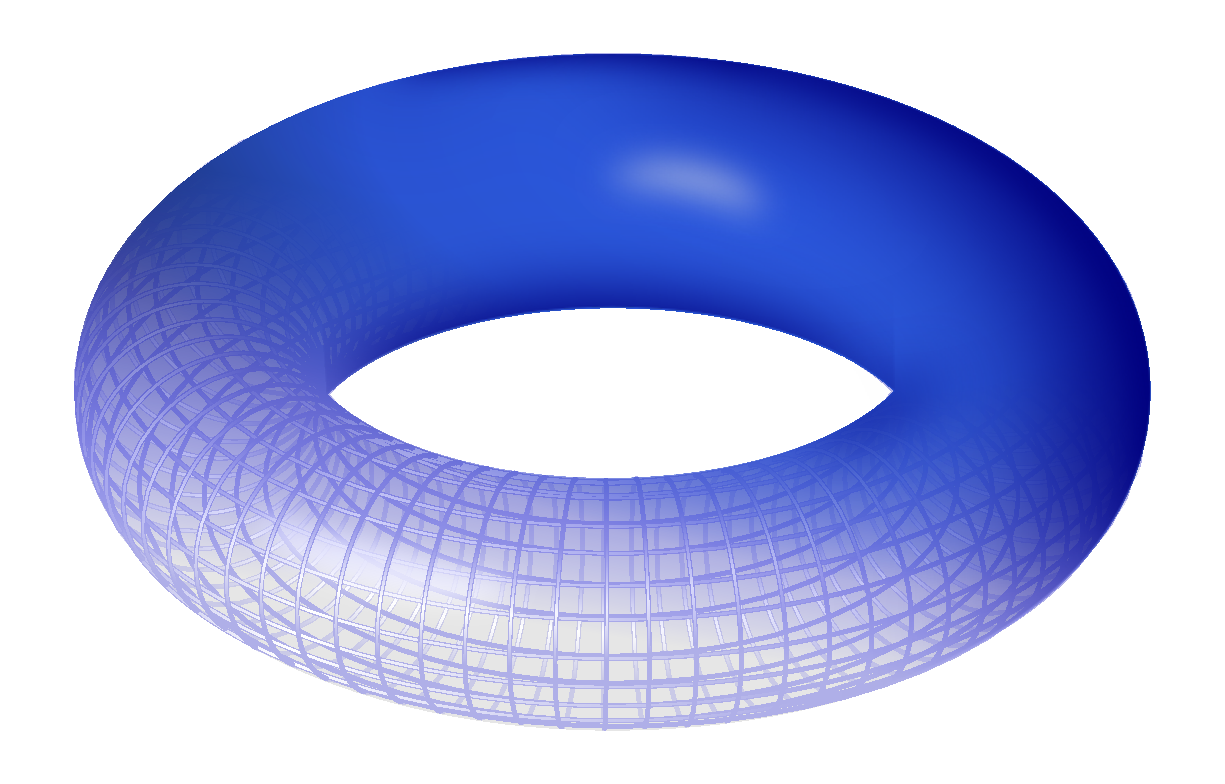
\includegraphics[width=0.35\textwidth ]{images/toro.pdf}
    \caption{Rappresentazione geometrica del toro $T^2$}
    \label{img:toro}
\end{figure}
\bigskip

\noindent\textbf{Esempio 7} Gli esempi precedenti consideravano varietà ''immerse'' in $\R^n$, il seguente esempio riguarda una varietà differenziabile che non nasce come sotto varietà contenuta in $\R^n$. Lo spazio \textbf{proiettivo reale} di dimensione $n$ si può costruire come segue, si consideri la seguente relazione di equivalenza fra vettori in $\R^{n+1}\backslash\{\mathbf 0\}$:\begin{equation}
    (x^0,x^1\dots,x^n)\sim(y^0,y^1\dots,y^n)\iff (y^0,y^1\dots,y^n)=(\lambda x^0,\lambda x^1\dots,\lambda x^n) \ \forall \lambda\ne 0.
\end{equation}
Si considera l'insieme quoziente delle classi di equivalenza rispetto tale relazione\begin{equation}
    \mathbb P^n_{\mathbb R}=\frac{\mathbb R^{n+1}\backslash\{\mathbf 0\}}{\sim}
\end{equation}
si denota $(x^0:x^1\dots : x^n)$ un'elemento di $\mathbb P^n_{\mathbb R}$. Dal punto di vista geometrico, ogni elemento di $\mathbb P^n_{\mathbb R}$ è una retta passante per l'origine, come mostrato in figura \ref{img:spazio_proiettivo}.
\begin{figure}[h!]
    \center
    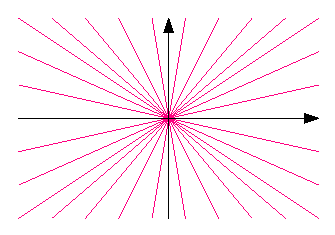
\includegraphics[width=0.35\textwidth ]{images/spazio_proiettivo.eps}
    \caption{Lo spazio $\mathbb P^1_{\mathbb R}$}
    \label{img:spazio_proiettivo}
\end{figure}

I punti  $(x^0:x^1\dots : x^n)$ si denominano \textbf{coordinate omogenee} in $\mathbb P^n$ (da ora in poi si omette il pedice $\mathbb R$). Lo spazio proiettivo deve essere dotato di una topologia, siccome $\mathbb P^n$ è un'insieme quoziente, è quindi dotato della \textit{topologia quoziente}, ai fini dell'esempio, non è necessario conoscere i dettagli di tale topologia.\bigskip

Si vuole ora costruire un atlante per $\mathbb P^n$, si pone\begin{equation}
    U_i=\{(x^0:x^1\dots : x^n)\in \mathbb P^n \ : \ x^i\ne 0\}
\end{equation}
di tali insiemi $U_i$ ce ne sono $n+1$, per $i=0,1\dots n$. Si ha che \begin{equation}
    \mathbb P^n=\bigcup_{0\le i\le n}U_i
\end{equation}
ogni punto dello spazio proiettivo deve avere almeno una coordinata diversa da zero, quindi deve essere necessariamente in uno degli insiemi $U_i$. Bisogna definire ora le carte locali, si pone $\varphi_i:U_i\rightarrow\R^n$ come segue\begin{equation}
    \varphi_i(x^0:\dots:x^n)=\big(
    \frac{x^0}{x_i},\dots \frac{x^{i-1}}{x_i},\frac{x^{i+1}}{x_i} ,\dots\frac{x^{n}}{x_i}       
    \big)
\end{equation}
nell'immagine di $\varphi_i$ si è esclusa la coordinata $x_i$, $\varphi_i$ è ben definita in quanto \begin{equation}
    \varphi_i(x^0:\dots:x^n)=\varphi_i(\lambda x^0:\dots:\lambda x^n)
\end{equation}
non è difficile da verificare\begin{align}
    &\varphi_i(\lambda x^0:\dots:\lambda x^n)=\big(
    \frac{\lambda x^0}{\lambda x_i},\dots \frac{\lambda x^{i-1}}{\lambda x_i},\frac{\lambda x^{i+1}}{\lambda x_i} ,\dots\frac{\lambda x^{n}}{\lambda x_i}       
    \big)=\\&\big(
    \frac{x^0}{x_i},\dots \frac{x^{i-1}}{x_i},\frac{x^{i+1}}{x_i} ,\dots\frac{x^{n}}{x_i}       
    \big)=\varphi_i(x^0:\dots:x^n).
\end{align}
La funzione inversa è la seguente\begin{align}
    &\varphi_i^{-1}:\R^n\rightarrow U_i\\ 
    &(y^1\dots,y^n)\longmapsto (y^1:\dots:y^i:1:y^{i+1}:\dots : y^n)
\end{align}
l'insieme $\{(U_i,\varphi_i)\}_{i=0,\dots n}$ è un atlante per $\mathbb P^n$. Bisogna verificare ora la regolarità delle funzioni di transizione. Siano $(U_i,\varphi_i),(U_j,\varphi_j)$ due carte, si considera $\eta_{ij}$:\begin{eqnarray}
    \eta_{ij}(y^1\dots,y^n)=\\
    \varphi_i\circ\varphi_j^{-1}(y^1\dots,y^n)=\\
    \varphi_i(y^1:\dots:y^j:1:y^{j+1}:\dots : y^n)=\\ 
    \big(
    \frac{y^1}{y^i}:\dots :   \frac{y^{i-1}}{y^i}  :\frac{y^{i+1}}{y^i}  :\dots :  
    \frac{y^{j}}{y^i} :\frac{1}{y^i}  :\frac{y^{j+1}}{y^i} :\dots : \frac{y^{n}}{y^i} 
    \big)
\end{eqnarray}
essendo che $y^i\ne 0 \ne y^j$, ogni funzione di transizione $\eta_{ij}$ è di classe $C^\infty$. In conclusione, $\mathbb P^n$ è una $n$-varietà differenziabile.\begin{osservazione}
    $\mathbb P^n_\R$ è l'insieme dei sotto spazi vettoriali di dimensione $1$ di $\R^{n+1}$, dato che contiene tutte le rette passanti per l'origine.
\end{osservazione}
Tale struttura si può generalizzare, sia $V$ uno spazio vettoriale sul campo reale di dimensione $n$, si definisce\begin{equation}
    Gr_k(V)=\{\text{ insieme dei sottospazi di }V\text{ di dimensione }k\}
\end{equation}
si ha che $\mathbb P^n_\R=Gr_{1}(\R^{n+1})$. L'insieme $Gr_{2}(\R^{n+1})$ contiene tutti gli iperpiani passanti per l'origine. Anche $Gr_k(V)$ è una varietà differenziabile di dimensione $k(n-k)$ ed è detta \textit{varietà grassmanniana}.
\subsection{Il Teorema degli Insiemi di Livello}
Il teorema presentato in tale sezione è rilevante. Sono necessari prima alcuni risultati, ed alcune definizioni.\begin{definizione}
    Sia $\Omega\subset\R^n$ un'aperto e sia $F:\Omega\rightarrow\R^m$ una funzione di classe $C^1$. Un punto $p\in\Omega$ è un \textbf{punto critico} di $F$ se il differenziale $dF_p:\R^n\rightarrow\R^m$ non è suriettivo (il rango della matrice Jacobiana in tal punto non è $m$). Il punto $F(p)$ è detto \textbf{valore critico}.
\end{definizione}
Sia $Crit(F)\subset\Omega$ l'insieme dei punti critici di $F$, tale insieme è chiuso (la dimostrazione è omessa). Si ricordi che nel caso $m=1$, un punto critico è un punto in cui il gradiente di $F$ si annulla. Se $n=m$, un punto è critico se la matrice Jacobiana ha determinante nullo.

Un punto è regolare se non è critico, e la sua immagine tramite $F$ è un valore regolare.
\begin{teorema}\label{teo:func_inv}\textbf{(della funzione inversa)}
Sia $\Omega\subset\R^n$ un aperto, e $F:\Omega\rightarrow\R^n$ una funzione di classe $C^k$ con $k\ge 1$. Sia $p_0\in\Omega$ un punto regolare, ossia $\det(\text{Jac}F(p_0))\ne 0$, esiste un'intorno $U$ di $p_0$ ed un'intorno $V$ di $F(p_0)$ in $\R^n$ tali per cui la funzione \begin{equation}
    F_{|U}:U\rightarrow V 
\end{equation}
è un diffeomorfismo (essa e la sua inversa sono differenziabili) la cui inversa è di classe $C^k$.
\end{teorema}
Intuitivamente, il teorema afferma che, se una funzione $F$ in un punto $p_0$ è approssimabile da un'applicazione lineare invertibile, anche $F$ stessa sarà localmente invertibile in un intorno di $p_0$.\bigskip

Il seguente teorema è fondamentale ed afferma che le curve di livello di una funzione di classe $C^\infty$ sono varietà differenziabili.
\begin{teorema}
    Sia $\Omega\subset\R^{m+n}$ un aperto, e sia \begin{equation}
        F:\Omega\rightarrow\R^m
    \end{equation} una funzione di classe $C^\infty$. Sia $a\in F(\Omega)$, si consideri l'insieme di livello di $a$, ossia l'insieme dei punti in $\Omega$ in cui la funzione assume valore $a$, escludendo i punti critici:\begin{align}
       &F^{-1}(a)=\{x\in\Omega \ : \ F(x)=a\}\\
        & M_a=F^{-1}(a)\backslash Crit(F)
    \end{align}
    allora $M_a$ è uno spazio topologico, la cui topologia è quella indotta da $\R^{m+n}$, inoltre è una $n$-varietà differenziabile. Se $a$ è regolare, $M_a=F^{-1}(a)$.
\end{teorema}
\textit{Dimostrazione}: Bisogna costruire un atlante per $M_a$, e mostrare che le funzioni di transizione sono di classe $C^\infty$. Si consideri un punto $p_0\in M_a$, siccome tale punto non è critico (per ipotesi), la matrice Jacobiana $\text{Jac}F(p_0)$ ha rango massimo, ossia $m$. Questo significa che esiste almeno una sotto-matrice di $\text{Jac}F(p_0)$ costituita da $n$ righe ed $m$ colonne che ha determinante diverso da zero. A meno di permutare le coordinate, si può assumere che queste siano le ultime $m$ colonne\begin{equation}\label{eq:jacobiana_G}
    \det\begin{pmatrix}
        \frac{\partial F^1}{\partial x^{n+1}(p_0)}&\dots& \frac{\partial F^1}{\partial x^{n+m}(p_0)}\\ 
        \vdots & & \vdots \\ 
        \frac{\partial F^m}{\partial x^{n+1}(p_0)}&\dots& \frac{\partial F^m}{\partial x^{n+m}(p_0)}
    \end{pmatrix}\ne 0
\end{equation}
denotiamo tale matrice $B$, essa è invertibile. Si costruisce una funzione $G:\Omega\rightarrow\R^{n+m}$ definita ponendo \begin{equation}
    G(x)=(x^1,\dots,x^n,F(x)).
\end{equation}
si considera poi la Jacobiana di $G$ in $p_0$\begin{equation}
    \text{Jac}G(p_0)=\begin{pmatrix}
        \text{Id}&\mathbf 0 \\ \mathbf * & B
    \end{pmatrix}
\end{equation}
è una matrice quadrata di $n+m$ righe e colonne, $\text{Jac}G(p_0)$ è suddivisa in quattro componenti come mostrato, in particolare\begin{itemize}
    \item $\text{Id}$ è la matrice identità, in quanto gli elementi di tali componenti sono del tipo \begin{equation}
        \frac{\partial x^i}{\partial x^j}
    \end{equation}
    e chiaramente, se $i=j$ allora $\frac{\partial x^i}{\partial x^j}=\frac{\partial x^i}{\partial x^i}=1$, differentemente, se $i\ne j$ si ha che $\frac{\partial x^i}{\partial x^j}=0$, quindi la matrice risultante è l'identità.
    \item La componente in alto a destra è la matrice nulla perché i termini sono tutti del tipo \begin{equation}
        \frac{\partial x^i}{\partial x^{n+j}}
    \end{equation}
    e per ogni $i,j$ tale derivata è nulla.
    \item La componente in basso a sinistra è composta dai termini del tipo 
    \begin{equation}
        \frac{\partial F^i}{\partial x^{n+j}}(p_0)
    \end{equation} 
    non vi sono assunzioni sui tali valori e con $\mathbf x$ si indica che tale matrice può assumere qualsiasi valore.
    \item L'ultima componente contiene termini del tipo\begin{equation}
        \frac{\partial F^i}{\partial x^{n+j}}
    \end{equation}
    ed è chiaramente la matrice $B$, come dall'equazione \eqref{eq:jacobiana_G}.
\end{itemize}
si conclude che il determinante di $\text{Jac}G(p_0)$ è uguale al determinante di $B$, quindi diverso da zero\begin{equation}
    \det\begin{pmatrix}
        \text{Id}&\mathbf 0 \\ \mathbf * & B
    \end{pmatrix}=\det B\ne 0.
\end{equation}
A tal punto si può applicare il Teorema \eqref{teo:func_inv}, $G$ è localmente invertibile, ossia esistono degli intorni $\tilde U\subset\Omega\backslash Crit(F)$ di $p_0$, e $W\subset\R^{n+m}$ di $G(p_0)$ tali che \begin{equation}
    G_{|\tilde U}:\tilde U \rightarrow W 
\end{equation}
è un diffeomorfismo. Sia $H$ l'inversa di $G_{|\tilde U}$\begin{equation}
    H(y)=(h^1(y),\dots h^{n+m}(y))
\end{equation}
essendo $H$ l'inversa di $G$ si ha che $G(H(y))=y$, in particolare\begin{eqnarray}
    y=(y^1,\dots y^{n+m})=G(H(y))=\\(h^1(y),\dots h^{n+m}(y),F(H(y)))
\end{eqnarray}
quindi per $i=1,2\dots,n$ si ha che $h^i(y)=y^i$. Pertanto\begin{eqnarray}
    F(H(y))=F(h^1(y),\dots,h^n(y),h^{n+1}(y),\dots h^{n+m}(y))=\\ 
    F(y^1,\dots,y^n,h^{n+1}(y),\dots h^{n+m}(y))
\end{eqnarray}
ma dato che $y=(h^1(y),\dots h^{n+m}(y),F(H(y)))$ si ha che l'ultimo blocco di $F(y^1,\dots,y^n,h^{n+1}(y),\dots h^{n+m}(y))$, ossia $h^{n+1}(y),\dots h^{n+m}(y)$, deve essere uguale all'ultimo blocco di $y$, quindi \begin{equation}
    F(H(y))=(y^{n+1}\dots, y^{n+m}) \ \ \forall y\in W
\end{equation}
Si pone $U=M_a\cap\tilde U$ e si definisce l'insieme \begin{equation}
    V=\{x\in\R^n \ : \ (x,a)\in W\}
\end{equation}
è un aperto di $\R^{n}$ dato che $W$ è un aperto di $\R^{n+m}$. Si definisce una funzione \begin{equation}
    \psi:V\rightarrow\R^{n+m}
\end{equation}
ponendo\begin{equation}
    \psi(x)=(x,h^{n+1}(x,a)\dots,h^{n+m}(x,a))
\end{equation}
dall'uguaglianza ricavata prima \begin{equation}
    F(y^1\dots,y^n,h^{n+1}(y)\dots ,h^{n+m}(y))=(y^{n+1}\dots,y^{n+m})
\end{equation}
si deduce che $\psi(V)=U=M_a\cap\tilde U$\begin{equation}
    \psi:\R^n\supset V \rightarrow U \subset M_a\subset\R^{n+m}
\end{equation}
si pone $\varphi=\psi^{-1}$, questa è una carta locale su $M_a$, definita su un'intorno $U$ di $p_0$. Tale costruzione può avvenire per ogni punto $p_0$, per tanto questo definisce un'atlante, $M_a$ è quindi una varietà topologica. Bisogna ora mostrare che le funzioni di transizione siano differenziabili.\bigskip

Siano $(U,\varphi)$ e $(U',\varphi')$ due carte, la funzione di transizione 
$\varphi'\circ\varphi^{-1}=\varphi'\circ\psi$ ha come coordinate termini del tipo $x^i$ oppure $h^j(x,a)$ (per 
costruzione), queste funzioni sono quindi di classe $C^\infty$.\hfill$\blacksquare$\bigskip

Saranno presi in considerazione alcuni esempi di applicazione di tale teorema. Sia $F:\R^{n+1}\rightarrow\R$ la seguente funzione:\begin{equation}
    F(x)=(\|x\|_2)^2
\end{equation}
ossia la funzione che associa ad ogni vettore la sua norma euclidea elevata al quadrato. La funzione è chiaramente di classe $C^\infty$, l'unico valore critico è $x=\mathbf 0$, in ogni altro punto, la matrice Jacobiana ha determinante diverso da zero, quindi per ogni $R\ne 0$ l'insieme di livello\begin{equation}
    F^{-1}(R^2)=S^n_R
\end{equation}
è una $((n+1)-1)$-varietà (è la sfera di raggio $R$). La dimensione della varietà è la differenza fra la dimensione del dominio con quella del codominio.\bigskip

\noindent Si consideri ora la funzione $F:M_n(\R)\simeq\R^{n^2}\rightarrow\R$ che assegna ad ogni matrice quadrata il suo determinante\begin{equation}
    F(A)=\det A.
\end{equation}
Sia $X=(x_i^j)\in M_n(\R)$, il determinante si calcola tramite lo sviluppo di Laplace:\begin{equation}
    \det X=\sum_{j=1}^n(-1)^{i+j}x_{i}^j\det X_i^j
\end{equation}
dove $X_i^j$ è la sotto-matrice di $X$ ottenuta eliminando la $i$-esima riga e la $j$-esima colonna. Da tale formula, si deduce che la derivata parziale di $F$ è la seguente\begin{equation}
    \frac{\partial F}{\partial x_i^j}=(-1)^{i+j}\det X_i^j
\end{equation}
Il differenziale di questa funzione non è suriettivo sui punti critici, essendo il codominio di dimensione 1, il differenziale non è suriettivo se la matrice Jacobiana ha rango zero, ossia è la funzione nulla, in tal caso i punti critici di $F$ sono le matrici che hanno derivate parziali nulle, $X$ è un punto critico se tutte le sotto-matrici $X_i^j$ hanno determinante nullo\begin{equation}
    X\text{ è critico }\iff \det X_i^j=0 \ \forall i,j.
\end{equation}
Ciò avviene se il rango di $X$ è minore o uguale di $n-2$\begin{equation}
    Crit(F)=\{X\in M_2(\R) \ : \ rk(X)\le n-2\}.
\end{equation}
Il determinante di una matrice quadrata di rango non massimo è nullo, quindi l'unico valore critico di $F$ è zero\begin{equation}
    \forall X\in Crit(F), \ F(X)=\det X=0.
\end{equation}
Si consideri un valore non critico, ad esempio 1, l'insieme di livello\begin{equation}
    SL(n,\R)=F^{-1}(1)=\{X\in M_2(\R) \ : \ \det X=1\}
\end{equation}
questo è il gruppo speciale lineare, è una varietà differenziabile di dimensione $n^2-1$.\bigskip

Tale teorema seppur potente nel suo enunciato va utilizzato in maniera corretta, si considerino le seguenti funzioni $F:\R^2\rightarrow\R$ e $G:\R^2\rightarrow\R$:\begin{align}
    & F(x,y)=y\\
    & G(x,y)=y^2
\end{align}
condividono l'insieme di livello per il valore 0:\begin{align}
    &F^{-1}(0)=\{(x,y) \ : \ y=0\}\\ 
    &G^{-1}(0)=\{(x,y) \ : \ y^2=0\}=\{(x,y) \ : \ y=0\}.
\end{align}
$F^{-1}(0)=G^{-1}(0)$ indica la retta di equazione $y=0$ ed è una 1-varietà. Il Jacobiano di $F$ è costante ed è Jac$F=(0,1)$, il rango è 1, non ci sono quindi valori critici per $F$.\bigskip 

Il Jacobiano di $G$ è Jac$G=(0,2y)$, ha rango nullo ove $y=0$, 0 è quindi un valore critico per $G$, il teorema non si può applicare  per $G^{-1}(0)$ perchè il valore non deve essere critico, nonostante ciò, questo insieme è comunque una varietà.\bigskip

Le funzioni $F$ e $G$ hanno lo stesso insieme di livello per il valore 0 il teorema enuncia che\begin{quote}
    l'antimmagine di un valore regolare è una varietà
\end{quote}
non dice che \begin{quote}
    l'antimmagine di un valore critico non è una varietà
\end{quote}
quest'ultima condizione si può comunque verificare.
\section{Funzioni Differenziabili fra Varietà}
Si considerino due varietà differenziabili $X,Y$, di dimensioni $n$ ed $m$. Sia $F$ una funzione continua\begin{equation}
    F:X\rightarrow Y
\end{equation}
si vuole definire il concetto di funzione di classe $C^r$ fra due varietà differenziabili. Ci si riconduce sempre ad insiemi aperti di $\R^n$, si considerino due carte per $X$ e per $Y$:\begin{align}
    &(U,\varphi) \text{ carta per }X, \ \ p\in U\\ 
    &(V,\psi) \text{ carta per }Y, \ \ q\in V
\end{align}
si considera $\tilde F$ la rappresentazione locale di $F$:
\[
\begin{tikzcd}
X \supset U \arrow[r, "F_{|U}"] \arrow[d, "\varphi"] & V \subset Y \arrow[d, "\psi"] \\
\mathbb{R}^m \supset \varphi(U) \arrow[r, "\widetilde{F}"] & \psi(V) \subset \mathbb{R}^m
\end{tikzcd}
\]
si ha che\begin{equation}
    \tilde F = \psi\circ F\circ\varphi^{-1}.
\end{equation}
$\tilde F$ è una funzione definita su un'aperto di $\R^n$ ad immagine su un'aperto di $\R^m$. 
\begin{definizione}\label{def:func_diff}
    Una funzione $F$ definita fra due varietà differenziabili è di classe $C^r$ in un'intorno di $p\in U$ se la sua rappresentazione locale $\tilde F$ è di classe $C^r$ in un'intorno di $q\in \varphi(p)$.
\end{definizione}
La definizione è ben posta se non dipende dalla scelta delle carte locali.

Si considerino due carte per $X$ $(U_1,\varphi_1),(U_2,\varphi_2)$ con $p\in U_1\cap U_2$. Siano $(V_1,\psi_1),(V_2,\psi_2)$ due carte per $Y$, con $q=F(p)\in V_1\cap V_2$. Si ha che
\[
\begin{tikzcd}[column sep=huge, row sep=huge]
\varphi_1(U_1 \cap U_2) \arrow[r, "\tilde F_1"] & \psi_1(V_1 \cap V_2) \\
U_1 \cap U_2\arrow[u, "\varphi_1"'] \arrow[d, "\varphi_2"'] \arrow[r, "F_{|U_1 \cap U_2}"] & V_1 \cap V_2 \arrow[d, "\psi_2"']\arrow[u, "\psi_1"']  \\
\varphi_2(U_1 \cap U_2) \arrow[r, "\tilde{F}_2"] & \psi_2(V_1 \cap V_2)
\arrow[from=3-1, to=1-1, bend left=50, looseness=1.5, "\varphi_1 \circ \varphi_2^{-1} = \eta{12}"{above, xshift=-1cm}, red]
\arrow[from=3-2, to=1-2, bend right=50, looseness=1.5, "\vartheta_{12} = \psi_1 \circ \psi_2^{-1}"{below, xshift=1cm}, red]
\end{tikzcd}
\]
$F$ ha due rappresentazioni locali, $\tilde F_1$ e $\tilde F_2$, sono tali che:\begin{equation}
    \tilde F_2=\vartheta_{12}^{-1}\circ\tilde F_1\circ\eta_{12}.
\end{equation}
La Definizione \ref{def:func_diff} è ben posta se, ogni qual volta una rappresentazione locale di $F$ ha una certa regolarità (è di classe $C^r$), allora anche una sua altra rappresentazione deve esserlo, siccome queste sono collegate dalle funzioni di transizione, l'unico modo per garantire ciò è che le funzioni di transizione siano a loro volta di classe $C^r$, ma queste per definizione di varietà differenziabile sono di classe $C^\infty$.\begin{definizione}
    Una funzione $F:X\rightarrow Y$ definita fra due varietà differenziabili è differenziabile se è di classe $C^\infty$ in ogni punto di $X$.
\end{definizione}
\begin{proposizione}
Siano $X,Y,Z$ tre varietà differenziabili, e siano \begin{align}
    &F:X\rightarrow Y\\ 
    &G:Y\rightarrow Z
\end{align}
funzioni differenziabili, allora\begin{equation}
    G\circ F:X\rightarrow Z 
\end{equation}
è differenziabile.
\end{proposizione}
\begin{definizione}
    Una funzione $F:X\rightarrow Y$
 fra varietà differenziabili è un diffeomorfismo di classe $C^r$ se è biettiva, di classe $C^r$, e la sua inversa è di classe $C^r$. Se non specificato, un diffeomorfismo è inteso di classe $C^\infty$. \end{definizione}
 \textbf{Esempio} Si consideri la varietà\begin{equation}
    X=GL(n,\R)=\{A\in M(n,\R) \ : \ \det A\ne 0\}
 \end{equation}
 è di dimensione $n^2$, la varietà $X\times X$ è di dimensione $2n^2$. L'applicazione\begin{align}
   & F:X\times X\rightarrow X\\ 
   &F(A,B)=A\cdot B
 \end{align}
 che associa a due matrici il loro prodotto\begin{align}
    &C=A\cdot B\\ 
    &c_j^i=\sum_h a_h^ib_j^h
 \end{align}
 le componenti di $F$ sono funzioni polinomiali, quindi $F$ è di classe $C^\infty$, pertanto è differenziabile.\bigskip

 Si consideri ora la funzione $G:X\rightarrow X$ definita come segue\begin{equation}
    G(A)=A^{-1}
 \end{equation}
 per le stesse ragioni, $G$ è differenziabile. Le funzioni $F$ e $G$ determinano il \textit{gruppo moltiplicativo} delle matrici quadrate a determinante non nullo, tali funzioni sono differenziabili, il gruppo $GL_n(\R)$ è un \textit{gruppo di Lie}.
 \begin{definizione}
    Un \textbf{gruppo di Lie} è un gruppo $G$, dotato di una struttura di varietà differenziabile, e per cui le funzioni che lo definiscono \begin{align}
        & G\times G\rightarrow G\text{ operazione binaria}\\ 
       & G\rightarrow G \text{ inverso}
    \end{align}
    sono entrambe differenziabili.
 \end{definizione}
 Il gruppo $(\R^n,+)$ è un gruppo di Lie.\bigskip

 \noindent\textbf{Esempio} Si consideri la varietà $X_1=\R$ (la retta reale) con unica carta $(U,\varphi)$ la funzione identità\begin{align}
    &\varphi:U\rightarrow \R\\ 
    &\varphi(x)=x\\ 
    &U=X_1.
 \end{align}
Si consideri poi $X_2=\R$  con unica carta $(V,\psi)$ la funzione cubica\begin{align}
    &\varphi:V\rightarrow \R\\ 
    &\varphi(x)=x^3\\ 
    &V=X_2.
 \end{align}
anche $X_2$ è la retta reale, ma dotata di una differente carta. Esistono varietà differenziabili diverse ma tra loro \textbf{diffeomorfe}, possono essere identificate da un diffeomorfismo, è il corrispettivo dell'isomorfismo fra gruppi. Due varietà sono uguali se diffeomorfe ed il diffeomorfismo che le mette in relazione è l'identità.\bigskip

$X_1$ e $X_2$ sono diverse perché l'identità non è un diffeomorfismo, si consideri però la funzione\begin{align}
    &F:X_1\rightarrow X_2\\
    &F(x)=\sqrt[3]{x}
\end{align}
questa è un diffeomorfismo:\begin{itemize}
    \item $F$ è biettiva
    \item $F$ è continua
\end{itemize}
la rappresentazione locale  $\tilde F$ è la funzione identità\begin{equation}
    \tilde F = x^3\circ \sqrt[3]{x}\circ x=x
\end{equation}
$\tilde F$ è chiaramente un diffeomorfismo.
\begin{osservazione}
    Come nell'Algebra si possono classificare i gruppi a meno di isomorfismi, si possono classificare le varietà differenziabili a meno di diffeomorfismi.
\end{osservazione}
In seguito, sono riportati alcuni risultati riguardanti la classificazione delle varietà differenziabili.\begin{itemize}
    \item Esistono varietà topologiche che non ammettono alcuna struttura differenziabile. Le varietà topologiche di dimensioni 1, 2 e 3 ammettono sempre una struttura differenziabile
    \item Le varietà topologiche di dimensioni 1, 2 e 3 ammettono un'unica struttura di differenziabile (a meno di diffeomorfismi).
    \item Se $n\ne 4$, la varietà $\R^n$ ammette un'unica struttura differenziabile a meno di diffeomorfismi. $\R^4$ è uno spazio topologico speciale perché ammette un'infinità non numerabile di strutture di varietà differenziabile. Si noti come lo spazio tempo in Relatività Generale è descritto come una $4$-varietà.
    \item La sfera unitaria $S^7$ ha 28 strutture differenziabili distinte non diffeomorfe e sono descritte tutte esplicitamente.
    \item Non è ancora noto quale sia il numero di strutture differenziabili distinte non diffeomorfe per $S^4$.
\end{itemize}
\begin{definizione}
    Una funzione $F:X\rightarrow Y$ è un \textbf{diffeomorfismo locale} se ogni $p\in X$ ha un'intorno aperto $U$ tale per cui $F(U)$ è aperto in $Y$ e la funzione\begin{equation}
        F_{|U}:U\rightarrow F(U)
    \end{equation}
    è un diffeomorfismo.
\end{definizione}
\begin{definizione}\label{def:rivestimento}
    Una funzione \begin{equation}
        \pi:\tilde X\rightarrow X 
    \end{equation}
    fra due varietà è un \textbf{rivestimento} se \begin{enumerate}
        \item $\pi$ è suriettiva e differenziabile
        \item per ogni $p\in X$ vi è un intorno aperto connesso $U\subset X$ tale per cui, per ogni componente connessa $\tilde U$
 di $\pi^{-1}(U)$, la restrizione $$ \pi_{|\tilde U}$$ è un diffeomorfismo fra $\tilde U$ e $U$.    \end{enumerate}
 Se $\tilde X$ è semplicemente connesso, $\pi$ è un rivestimento universale.
\end{definizione}
Un'esempio è il seguente, siano\begin{align}
    &\tilde X =\R\\ 
    &X=S_R^1\subset \R^2\\
    &\pi : \tilde X\rightarrow X\\ 
    &\pi(t)=(R\cos t,R\sin t)
\end{align}
$\pi$ è un rivestimento universale.
\subsection{Esempi di Gruppi di Lie}
Si consideri $\R^2$, questo si può identificare come il campo dei numeri complessi, ereditandone la struttura$\C$\begin{equation}
    (a,b)\longleftrightarrow z=a+ib
\end{equation}
inoltre\begin{equation}
    U(1)=\{z\in\C \ : \ |z|=1\}=\{(a,b)\in\R^2 \ : \ a^2+b^2=1\}=S^1
\end{equation}
$U(1)$ è un gruppo rispetto l'operazione di prodotto (il prodotto di due numeri complessi di norma unitaria è un numero di norma unitaria). $S^1$ eredita da $U(1)$ la struttura di gruppo abeliano (è un gruppo di Lie commutativo).\bigskip

Si consideri $\R^4$ questo si identifica come l'insieme dei quaternioni \begin{align}
    &\R^4\simeq\mathbb H\\ 
    &(a,b,c,d)\longleftrightarrow z= a+bi+cj+dk
\end{align}
dove\begin{align}
    &i^2=j^2=j^2=-1, \ ij=k, \ ji=-k, \ \text{ecc.}
\end{align}
il prodotto nell'insieme $\mathbb H$ non è commutativo. Il modulo per un quaternione si definisce come segue:\begin{equation}
|z|^2=z\cdot\overline z=(a+bi+cj+dk)(a-bi-cj-dk)=a^2+b^2+c^2+d^2
\end{equation} Il gruppo dei quaternioni unitari identifica la sfera $S^3$\begin{equation}
    \{z\in\mathbb H \ : \ |z|=1\}=\{(a,b,c,d)\in\R^4 \ : \ a^2+b^2+c^2+d^2=1\}=S^3
\end{equation}
$S^3$ eredita dal gruppo dei quaternioni unitari una struttura di gruppo di Lie non abeliano.\bigskip

\noindent
Si considerino adesso le tre \textbf{matrici di Pauli}:\begin{equation}
    \sigma_X=\begin{pmatrix}
        0&1\\1&0
    \end{pmatrix} \ \ \ 
    \sigma_Y=\begin{pmatrix}
        0&-i\\i&0
    \end{pmatrix} \ \ \ 
    \sigma_Z=\begin{pmatrix}
        1&0\\0&-1
    \end{pmatrix} 
\end{equation}
sono matrici complesse ed unitarie (svolgono un ruolo fondamentale nel calcolo quantistico). Si ha che\begin{equation}
    \sigma_X^2=\sigma_Y^2=\sigma_Z^2=I=\begin{pmatrix}
        1&0\\0&1
    \end{pmatrix}
\end{equation}
inoltre\begin{equation}
    \sigma_X\sigma_Y=i\sigma_Z, \ \  \sigma_Y\sigma_X=-i\sigma_Z, \ \ \text{ecc.}
\end{equation}
Se si moltiplica ogni matrice per $i$ si costruiscono tre nuove matrici:\begin{equation}
\tilde\sigma_X=i\sigma_X \ \ \ 
    \tilde\sigma_Y=i\sigma_Y \ \ \ 
    \tilde\sigma_Z=i\sigma_Z
\end{equation}
queste soddisfano le seguenti relazioni\begin{align}
    &\tilde\sigma_X^2=\tilde\sigma_Y^2=\tilde\sigma_Z^2=-I\\
    &\tilde\sigma_X\tilde\sigma_Y=-\tilde\sigma_Z, \ \ \tilde\sigma_Y\tilde\sigma_X=\tilde\sigma_Z, \ \  
    \tilde\sigma_Y\tilde\sigma_Z=-\tilde\sigma_X \\ 
    & \tilde\sigma_Z\tilde\sigma_Y=\tilde\sigma_X, \ \ \tilde\sigma_X\tilde\sigma_Z=\tilde\sigma_Y, \ \  
    \tilde\sigma_Z\tilde\sigma_X=-\tilde\sigma_Y
\end{align}
confrontando tali relazioni con quelle dei quaternioni, si stabilisce la seguente corrispondenza\begin{align}
    &1\leftrightarrow I\\ 
    &i\leftrightarrow \tilde\sigma_Z\\
    &j\leftrightarrow \tilde\sigma_Y\\
    &k\leftrightarrow \tilde\sigma_X
\end{align}
i quaternioni si possono quindi rappresentare come delle matrici\begin{align}
    & z=a+bi+cj+dk\longleftrightarrow aI+b\tilde\sigma_Z+c\tilde\sigma_Y+d\tilde\sigma_X=\\ &\begin{pmatrix}
        a+ib&c+id\\ -c+id&a-ib
    \end{pmatrix} =A_z\in M(2,\C)
\end{align}
si noti che l'operazione di determinante è l'equivalente del modulo\begin{equation}
    \det A_z=(a+ib)(a-ib)-(c+id)(-c+id)=a^2+b^2+c^2+d^2
\end{equation}
vi è quindi una corrispondenza fra il gruppo dei quaternioni unitari ed il gruppo delle matrici $2\times 2$ unitarie a valori complessi $SU(2)$ con determinante uguale ad 1, in particolare, i due gruppi sono isomorfi. In conclusione: \begin{equation}
    SU(2)\simeq \{z\in\mathbb H \ : \ |z|=1\}\simeq S^3.
\end{equation}
\section{Quaternioni Unitari e Rotazioni}
Si consideri l'insieme dei quaternioni con prima coordinata nulla
\begin{equation}
    \quat_0=\{0+bi+cj+dk\}\subset\quat_0
\end{equation}
$\quat_0$ si può identificare con $\R^3$ tramite la seguente mappa $q:\R^3\rightarrow\quat_0$:\begin{equation}
    q(x^1,x^2,x^3)=x^1i+x^2j+x^3k.
\end{equation} 
Sia $z\in\quat$ un quaternione unitario, si definisce una trasformazione $R_z:\quat_0\rightarrow\quat_0$ come segue:\begin{align}
   & x\in\R^3\\
   & R_z(q(x))=zq(x)z^{-1}
\end{align}
il quaternione risultante avrà ancora parte reale nulla (facile da verificare). Siccome $\quat_0$ si identifica come $\R^3$, la funzione $R_z$ è identicamente una mappa fra vettori in $\R^3$. Si ha inoltre che la mappa $R_z$ è un'isometria di $\quat_0\simeq\R^3$:\begin{equation}
    |R_z(q(z))|=|zq(x)z^{-1}|=|z|\cdot|q(x)|\cdot|z^{-1}|=|q(x)|
\end{equation}
$R_z$ è un'applicazione lineare, ha determinante unitario\begin{equation}
    \det R_z=1
\end{equation}
la mappa $R_z:\R^3\rightarrow\R^3$ è una \textbf{rotazione} nello spazio $\forall z\in\quat, \ |z|=1$. Una rotazione si può sempre scrivere sotto forma di matrice (essendo lineare), se $z= a+bi+cj+dk$ con $|z|=1$, $R_z$ è rappresentata dalla seguente:\begin{equation}
    R_z = \begin{pmatrix}
a^2+b^2-c^2-d^2 & 2bc-2ad & 2bd+2ac \\
2bc+2ad & a^2-b^2+c^2-d^2 & 2cd-2ab \\
2bd-2ac & 2cd+2ab & a^2-b^2-c^2+d^2
\end{pmatrix}
\end{equation}
si dimostra che ogni rotazione in $\R^3$ è del tipo $R_z$ per qualche quaternione unitario $z$. Per ogni rotazione in $\R^3$ esistono esattamente due quaternioni unitari che la descrivono\begin{equation}
    R_z=R_z'\iff\begin{cases}
        z=z'\ \text{ oppure}\\z=-z'
    \end{cases}
\end{equation}
Ricapitolando:\begin{itemize}
    \item Ad ogni quaternione di modulo 1 si è associata una matrice $A_z\in M(2,\C)$ tramite una corrispondenza biettiva
    \item questa identifica il gruppo dei quaternioni unitari con il gruppo $SU(2)$.
    \item Ad ogni quaternione di modulo 1 si è associata una matrice di rotazione $R_z\in SO(3)$ tramite una corrispondenza non biettiva
    \item si ricordi che $SO(3)$ è il gruppo delle matrici ortogonali con determinante uguale ad 1.
\end{itemize}
Questo è un \textbf{omomorfismo suriettivo} di gruppi di Lie. Il nucleo dell'omomorfismo è $\{-I,I\}$:\begin{equation}\label{eq:SU2-SO3}
    \frac{SU(2)}{\{I,-I\}}\simeq SO(3)
\end{equation}
$SU(2)$ e $SO(3)$ hanno una struttura di varietà differenziabile. Si noti come $SU(2)\simeq S^3$ è semplicemente connesso, quindi $SU(2)$ è il \textit{rivestimento universale} di $SO(3)$.\bigskip

Dall'equazione \eqref{eq:SU2-SO3}, si ha che prendere il quoziente di $S^3$ rispetto il sottogruppo $\{I,-I\}$ significa identificare punti diametralmente opposti su $S^3$, ma le coppie di punti diametralmente opposti sulla sfera rappresentano lo spazio proiettivo $\mathbb P^3_\R$, considerando la relazione $\sim$ fra due punti su $S^3$\begin{equation}
x\sim y\iff x=-y
\end{equation} si hanno pertanto i seguenti diffeomorfismi:\begin{equation}
    \mathbb  P^3_\R\simeq \frac{S^3}{\sim}\simeq  \frac{SU(2)}{\{I,-I\}}\simeq SO(3).
\end{equation}



\chapter{Lo Spazio Tangente}
Si vuole definire il concetto di \textit{vettore tangente} ad una varietà in un suo punto.
\begin{figure}[h!]
    \center
    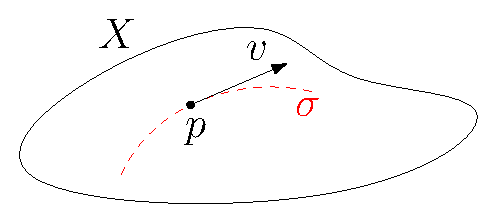
\includegraphics[width=0.4\textwidth ]{images/vettore_tangente.eps}
    \caption{Vettore tangente ad un punto di $X$}
    \label{img:vec_tang}
\end{figure}

L'idea è quella di rappresentare un vettore tangente ad una varietà $X$ in un punto $p$ come vettore tangente ad un'arco di curva $\gamma$ contenuta in $X$ passante per $p$, come mostrato in figura \ref{img:vec_tang}. Tale idea va formalizzata utilizzando le carte locali di $X$. Tale idea è poco elegante dato che il vettore tangente in questo caso dipenderà dalla scelta della carta, va quindi considerato un'altro approccio.\section{Lo Spazio delle Derivazioni}
Per spiegare l'idea si comincia con un caso semplice, si consideri la varietà $X=\R^n$. Dato un qualsiasi punto $p\in\R^n$, lo spazio tangente a tale punto, denotato $T_p\R^n$, è esattamente $\R^n$.\bigskip

La definizione formale di spazio tangente sarà data in seguito, considerando la definizione poco elegante, è chiaro che nel caso di $\R^n$, una qualsiasi curva passante per un punto può identificare un qualsiasi vettore tangente.
\bigskip

Sia $v\in T_p\R^n\in\R^n$ un vettore tangente e sia $f$ una funzione di classe $C^\infty$ definita in un'intorno di $P$.
Si può calcolare la \textbf{derivata direzionale} di $f$ in $p$ rispetto al vettore $v$:\begin{align}
    &v=(a^1,a^2\dots,a^n)\in T_p\R^n\\
    &\partial_vf(p)=\sum_{i=1}^n a^i\frac{\partial f}{\partial x_i}(p)
\end{align}
Si consideri ora l'insieme delle funzioni a valori reali derivabili infinite volte in $p$\begin{equation}
    C_p^\infty=\{f:U\rightarrow\R \ : \ f\text{ è di classe }C^\infty \text{ in un'intorno aperto }U\text{ di }p\}
\end{equation}
la derivata direzionale valutata in $p$ è un'operatore da $ C_p^\infty$ ad $\R$\begin{align}
    &\partial_{v_{|p}}: C_p^\infty\rightarrow\R\\ 
    &f\longmapsto \partial_vf(p)
\end{align}
questa soddisfa le seguenti proprietà\begin{itemize}
    \item $\partial_{v_{|p}}(f+g)=\partial_{v_{|p}}(f)+\partial_{v_{|p}}(g)$
    \item $\partial_{v_{|p}}(\text{costante})=0$
    \item $\partial_{v_{|p}}(fg)=\partial_{v_{|p}}(f)g(p)+f(p)\partial_{v_{|p}}(g)$ \textbf{regola di Leibniz}.
\end{itemize}
\begin{definizione}
    Un'operatore $D: C_p^\infty\rightarrow\R$ che soddisfa le tre proprietà elencate in un punto $p$ è detto \textbf{derivazione centrata} in $p$.
\end{definizione}
Si denota $Der_p$ l'insieme di tali derivazioni. Ad ogni vettore di $\R^n$ risulta associata una di queste derivazioni, $Der_p$ ha la proprietà di essere uno spazio vettoriale sul campo dei reali, de facto \begin{align}
    &D_1,D_2\in Der_p\implies D_1+D_2\in Der_p\\ 
    & D\in Der_p,\lambda\in\R\implies \lambda D\in Der_p
\end{align}
Ritornando alla varietà $X=\R^n$ e allo spazio tangente $T_pX$, ad ogni vettore $v=(a^1,a^2\dots,a^n)$ in tale spazio, è associata una derivazione centrata in $p$:\begin{equation}
    \partial_{v_{|p}}={\sum_{i=1}^n a^i\frac{\partial }{\partial x_i}}\hphantom{.}_{|p}\in Der_p
\end{equation}
questa associazione è lineare ed è un'omeomorfismo fra spazi vettoriali\begin{align}
    &T_p\R^n\rightarrow Der_p\\ 
    & v\longmapsto  \partial_{v_{|p}}
\end{align}
Questo spazio vettoriale è relativo ad un punto $p$. Ad ogni punto $p$ si può associare uno spazio vettoriale  $T_p\R^n$. Si vedrà in seguito che in realtà tale omeomorfismo è un'isomorfismo, gli spazi vettoriali $T_p\R^n, Der_p$ si possono identificare, in tal modo lo spazio vettoriale delle derivazioni si può identificare con lo spazio tangente (almeno nel caso di $\R^n$).\bigskip

\noindent
Si comincia definendo in maniera più rigorosa $C^\infty_p$. Sia $X$ una varietà differenziabile, e $p\in X$, se $U\subset X$ è un'aperto, si pone\begin{equation}
    C^\infty(U)=\{f:U\rightarrow\R \ : \ f\text{ è di classe }C^\infty\}
\end{equation}
si considera l'insieme delle coppie $(U,f)$ tali per cui $U$ è un'aperto di $X$ contenente $p$ e $f\in C^\infty(U)$. Sull'insieme $\{(U,f)\}$ di tutte le coppie di questo tipo si definisce una relazione di equivalenza:\begin{equation}
    (U_1,f_1)\sim (U_2,f_2)\iff \begin{matrix}
        \exists W\text{ intorno aperto di }p\text{ tale che }\\W\subset U_1\cap U_2\text{ ove }f_{1_{|W}}=f_{2_{|W}}
    \end{matrix}
\end{equation}\begin{center}
    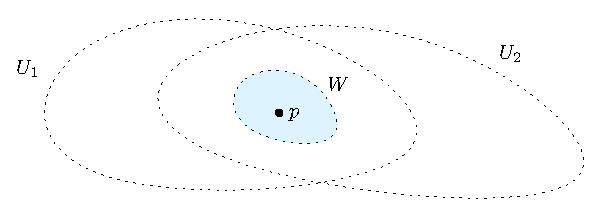
\includegraphics[width=0.4\textwidth ]{images/relazione_C.eps}
\end{center}
Si richiede che $f_1$ ed $f_2$ coincidano in un qualche intorno aperto $W$ di $p$.
\begin{definizione}
    Si pone\begin{equation}
        C_p^\infty=\frac{\{(U,f) \ : \ p\in U, f\in C^\infty(U)\}}{\sim}
    \end{equation}
    come insieme quoziente. Si indicherà $[(U,f)]\in  C_p^\infty$ una classe di equivalenza.
\end{definizione}
Si pone $f_p=[(U,f)]$ e si denomina \textbf{germe} di $f$ in $p$. Intuitivamente il germe di una funzione in un punto $p$ è semplicemente una funzione definita in un qualche intorno $U$ di $p$ che è di classe $C^\infty$.
Nell'insieme $C_p^\infty$ si possono definire somma e prodotto:\begin{align}
    &[(U_1,f_1)]+[(U_2,f_2)]=[[(U_1\cap U_2,f_1+f_2)]]\\
    &[(U_1,f_1)]\cdot[(U_2,f_2)]=[[(U_1\cap U_2,f_1 f_2)]].
\end{align}
$C_p^\infty$ ha una struttura di anello, si può verificare facilmente, è detto \textit{anello dei germi delle funzioni di classe $C^\infty$ in $p$}.\bigskip

\noindent
L'anello $C^\infty(U)$ prima definito, con $p\in U$, è omeomorfo a $C_p^\infty$ tramite la mappa:\begin{equation}
    f\longmapsto  f_p=[(U,f)]
\end{equation}
che associa ad una funzione $f$ il suo germe in $p$.
\begin{osservazione}
    Sia $F:X\rightarrow Y$ una funzione differenziabile fra due varietà, se $U\subset Y$, allora $F^{-1}(U)$ è un'aperto di $X$, dato che $F$ è continua, se $f\in C^{\infty}(U)$, ossia è di classe $C^\infty$ su $U$, allora è valido il seguente diagramma commutativo:
\end{osservazione}
\[
\begin{tikzcd}
X \supset F^{-1}(U) \arrow[rr, "F"] \arrow[dr, "f \circ F"'] & & U \subset Y \arrow[dl, "f"] \\
& \mathbb{R} &
\end{tikzcd}
\]
Dato che $f$ e $F$ sono di classe $C^\infty$, lo è anche $f\circ F$ nell'insieme $F^{-1}(U)$. Per ogni aperto $U\subset Y$, la funzione $F:X\rightarrow Y$ induce una funzione $F^*$ come segue
\begin{align}
    &F^*:C^\infty(U)\rightarrow C^\infty(F^{-1}(U))\\
    &f\longmapsto F^*(f)=f\circ F
\end{align}
si verifica che $F^*$ è un'omomorfismo di anelli. Questo vale per ogni aperto $U$, vi è un'analoga funzione di $F^*$ definita sui germi delle funzioni, sia $p\in X$ e $q=F(p)\in Y$:\begin{align}
    &F_p^*:C^\infty_q\rightarrow C^\infty_p\\
    &[(U,f)]\longmapsto [(F^{-1}(U),f\circ F)].
\end{align}
La funzione $F^*$ è detta ''pull back''.\subsection{Lo Spazio Cotangente}
Si vuole definire in maniera ora formalmente il concetto di vettore tangente ad una varietà. La definizione di derivazione è stata già accennata:\begin{definizione}\label{def:derivazioni}
    Sia $X$ una varietà e $p\in X$. Una \textbf{derivazione} in $p$ è un'operatore \begin{equation}
        D:C^\infty_p\rightarrow \R  
    \end{equation}
    che soddisfa le seguenti proprietà:\begin{itemize}
        \item $D(f+g)=D(f)+D(g)$
        \item $D(\text{costante})=0$
        \item $D(fg)=D(f)g(p)+D(g)f(p), \ \ \forall f,g\in C_p^\infty$
    \end{itemize}
\end{definizione}
L'insieme delle derivazioni per $X$ in $p$ è denotato $Der_p$. Il numero reale associato è da intendersi come la derivata di una funzione del germe contenuto in $C^\infty_p$ calcolata in $p$.
\begin{definizione}
     Sia $X$ una varietà e $p\in X$. Lo \textbf{spazio tangente} a $X$ in $p$ è uno spazio vettoriale reale denotato $T_pX$ costituito da tutte le derivazioni di $X$\begin{equation}
        T_pX=Der_p.
     \end{equation}
\end{definizione}
Se $n$ è la dimensione della varietà $X$, $Der_p$ è isomorfo a $\R^n$. $T_pX$ è definito esclusivamente dalla varietà $X$ e da un punto $p$, e non dipende dalle carte locali.\bigskip

Si consideri un punto $p\in X$ di una varietà, ad ogni punto possiamo associare l'anello $C_p^\infty$, vogliamo però associare ad ogni punto uno spazio tangente. In $C_p^\infty$ potremmo considerare il sottoinsieme di  tutti i germi di funzioni che si annullano in $p$\begin{equation}
    C_p^\infty \supset m_p = \{f_p\in C_p^\infty \ :  \ f_p(p)=0 \}
\end{equation}
si ricordi che $f_p$ non è una funzione ma una classe di equivalenza $[(U,f)]$, dire $f_p(p)=0$ equivale a dire $f(p)=0$. $m_p$ è un \textbf{ideale}, perché è un sotto anello, ed un elemento di $m_p$ moltiplicato per un qualsiasi elemento di $ C_p^\infty$ produce un elemento a sua volta in  $m_p$:\begin{align}
    &f_p\in m_p\\ 
    &f'_p\in C_p^\infty \\ 
    &f_p(p)=0\in \R\\
    &f'_pf_p(p) =f_p(p)f'_p(p)=\\& 0\cdot f'_p(p)=0\implies\\
   & f'_p\in m_p.
\end{align}
$m_p$ è un modulo sull'anello $C_p^\infty$, se si prende il quoziente \begin{equation}
    \frac{m_p}{m_p^2}
\end{equation}
si ha un modulo sull'anello quoziente $\frac{C_p^\infty}{m_p}$. Tale quoziente è isomorfo a $\R$ (i dettagli verranno omessi), si ha una funzione $\phi:C_p^\infty\rightarrow \R$ definita\begin{equation}
    \phi(g_p)=g_p(p)
\end{equation}
il nucleo di questa funzione (gli elementi che la annullano) è esattamente $m_p$, per definizione\begin{equation}
    \ker\phi=m_p 
\end{equation} 
come detto prima, se si considera il quoziente  $C_p^\infty$ modulo il nucleo di $\phi$, si ottiene uno spazio isomorfo a $\R$. $\frac{m_p}{m_p^2}$ è un modulo sull'anello $\frac{C_p^\infty}{m_p}\simeq \R$, questo è un campo (il campo dei numeri reali), ma per definizione, un modulo su un campo è uno spazio vettoriale, conclusione:\begin{equation}
    \frac{m_p}{m_p^2}\text{ è uno spazio vettoriale reale}
\end{equation}
in particolare, è uno spazio associato in modo canonico al punto $p$. Questa è una definizione nei termini dell'algebra commutativa, non ne è necessario conoscere i dettagli (io stesso non l'ho compresa). Lo spazio $\frac{m_p}{m_p^2}$ non è lo spazio tangente $T_pX$, ma il suo spazio duale:\begin{equation}
     \frac{m_p}{m_p^2}\simeq \hom(T_pX,\R)=T_p^*X
\end{equation}
$ \frac{m_p}{m_p^2}=T_p^*X$ è detto lo \textbf{spazio cotangente}.\bigskip


\noindent\textbf{Nota}: Il fatto che la dimensione dello spazio tangente ad un punto di una varietà sia la stessa della varietà, va dimostrato.
\section{Derivazioni e Carte Locali}
Si introducono ora le carte locali nel contesto dello spazio tangente. Sia $(U,\varphi)$ una carta per una varietà $X$ tale per cui $p\in U$. Siano $(x^1\dots,x^n)\in\R^n$ le coordinate di $\varphi(p)$. Le coordinate cartesiane in $\R^n$ determinano delle derivazioni naturali rispetto tali coordinate (le derivate parziali)\begin{equation}
    \partial_1=\frac{\partial}{\partial x^1}, \ \partial_2=\frac{\partial}{\partial x^2}\dots,\partial_n=\frac{\partial}{\partial x^n}
\end{equation}
$\partial_i$ è la derivata nella direzione del versore determinato dall'asse $x^i$. Le derivate parziali corrispondo ad i versori degli assi, che sono la base canonica $(e_1,\dots,e_n)$ di $T_q\R^n\simeq\R^n$ per ogni $q\in\R^n$.\bigskip

\noindent Si vogliono definire delle derivazioni definite su $U\subset X$. Usando $\varphi$ si possono associare derivazioni definite su $X$ a derivazioni classiche su $\R^n$ (le derivate parziali). Sia \begin{equation}
    f_p=[(V,f)]\in C_p^\infty
\end{equation}
un germe nel punto $p$. Si può supporre che $V\subset U$ (dominio della carta locale), considerando eventualmente un'aperto più piccolo contenente $p$.
\[
\begin{tikzcd}[column sep=huge, row sep=huge]
U \supset V \arrow[r, "\varphi"'] \arrow[d, "f"'] & \varphi(V) \subset \mathbb{R}^n \arrow[dl, "f \circ \varphi^{-1}"'] \\
\mathbb{R}
\end{tikzcd}
\]
Si pone\begin{equation}\label{eq:derivata}
    \partial_{i_{|p}}(f_p)=\frac{\partial (f\circ\varphi^{-1})}{\partial x_i}(\varphi(p))
\end{equation}
$ \partial_{i_{|p}}(f_p)\in T_pX$ rappresenta il vettore tangente a $X$ lunga la curva che si ottiene come anti immagine del versore $x^i$ tramite la carta locale $\varphi$:\begin{itemize}
    \item In $\R^n$ vi è $\varphi(p)=(\varphi_1(p),\dots\varphi_n(p))(x^1\dots,x^n)$
    \item si consideri la curva $\gamma_i(t)=(x^1,x^2\dots,x^i+t\dots,x^n)$ che è una retta parallela all'$i$-esimo asse passante per $\varphi(p)$.
    \item si considera l'anti-immagine di questa curva $\gamma(t)$ tramite la carta locale, ossia la curva $\varphi^{-1}(\gamma(t))$, questa è una curva su $X$ passante per $p$
    \item il vettore $\partial_{i_{|p}}(f_p)$ è tangente a questa curva $\varphi^{-1}(\gamma(t))$ nel punto $p$ (ossia per $t=0$).  $\partial_{i_{|p}}(f_p)$  rappresenta la direzione in cui ''cambia'' la varietà quando ti muovi lungo la curva che corrisponde all'$i$-esimo asse coordinato locale. Una rappresentazione è riportata in figura \ref{img:derivata}.
\end{itemize}

\begin{figure}[h!]
    \center
    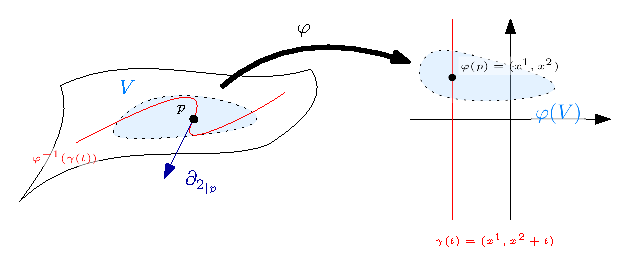
\includegraphics[width=0.7\textwidth ]{images/derivata.eps}
    \caption{Un esempio per una $2$-varietà.}
    \label{img:derivata}
\end{figure}

\begin{quote}
$ \partial_{i_{|p}}(f_p)$ è un numero reale che rappresenta la variazione della funzione $f_p=[(f,U)]$ lungo la curva $\varphi^{-1}(\gamma(t))$.
\end{quote}
Le funzioni $\partial_{i_{|p}}$ sono delle derivazioni, soddisfano le proprietà date nella Definizione \ref{def:derivazioni}, sono quindi i vettori tangenti (elementi dello spazio tangente $T_pX$). Gli operatori $\partial_{i_{|p}}$ dipendono dalla scelta di una carta locale $\varphi$, come si può notare dalla definizione in \eqref{eq:derivata}. L'analogo della derivata parziale sulla carta locale dipende dalla scelta della carta locale, l'unica cosa indipendente da tale scelta è lo spazio tangente in un punto $T_pX$.
\subsection{Differenziale di una Funzione fra Varietà}
Si consideri una funzione $F:X\rightarrow Y$ fra due varietà, sia $p\in X$ e $q=F(p)\in Y$. Si consideri un vettore $v\in T_pX$, $v$ è tangente ad un'arco di curva $\sigma\subset X$ ove $p\in\sigma$, tramite $F$, si identifica una curva $F(\sigma)\subset Y$, chiaramente $q\in F(\sigma)$ e vi sarà un vettore $w$ tangente a $q$ lungo la curva $F(\sigma)$.

\begin{center}
    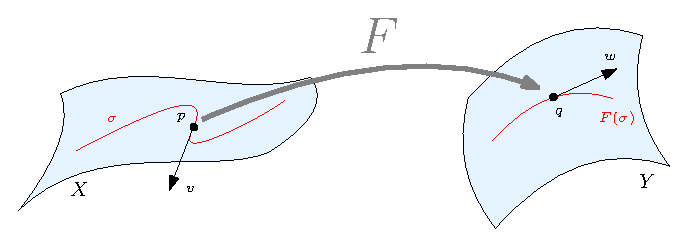
\includegraphics[width=0.7\textwidth ]{images/differenziale.eps}
\end{center}


\noindent La funzione $F$ induce una mappa (quella che associa $w$ a $v$) fra gli spazi tangenti $T_pX$ e $T_qY$. Tale mappa è detta \textbf{differenziale} di $F$ in $p$, ed è una funzione lineare fra spazi vettoriali. La definizione di differenziale sarà data interpretando $T_pX$ e $T_qY$ come gli spazi delle derivazioni.\bigskip

Si ricordi che $F$ induce una funzione $F^*_p$ che è un'omomorfismo di anelli:
\begin{align}
    &F_p^*:C^\infty_{F(p)}\rightarrow C^\infty_p\\
    &[(U,f)]\longmapsto f\circ F.
\end{align}
questa era il pull back, sia $D\in T_pX$ una derivazione, si ha il seguente diagramma:
\[
\begin{tikzcd}[column sep=huge, row sep=huge]
C^\infty_{F(p)} \arrow[r, "F_p^*"'] \arrow[d, "D\circ F_p^*"'] & C_p^\infty \arrow[dl, "D"'] \\
\R
\end{tikzcd}
\]
La funzione $D\circ F_p^*$ associa ad ogni germe di funzione un numero reale\begin{equation}
    D\circ F_p^*:C_{F(p)}^\infty\rightarrow\R
\end{equation}
Dato che $D$ è una derivazione, anche $D\circ F_p^*$ è una derivazione, si verifica facilmente:\begin{equation}
(D\circ F_p^*)(f)=D(F_p^*(f))=D(f\circ F).
\end{equation} L'applicazione lineare che associa elementi fra gli spazi tangenti (il differenziale di $F$) è la seguente\begin{align}
    & T_pX\rightarrow T_{F(p)}Y\\
    & D\longmapsto D\circ F_p^*
\end{align}
\begin{definizione}
    Sia $F:X\rightarrow Y$ una funzione fra due varietà differenziabili. Si definisce il \textbf{differenziale} di $F$ in un punto $p\in X$ la seguente applicazione lineare\begin{align}
        & dF_p:T_pX\longrightarrow T_{F(p)}Y\\
    & D\longmapsto dF_p(D)=D\circ F_p^*.
    \end{align}
    A volte si denota $T_pF$.
\end{definizione}
Vediamo adesso alcune proprietà del differenziale.
\begin{proposizione}
    \begin{enumerate}
    \item Sia $F$ la funzione identità su una varietà $X$\begin{equation}
        F=\text{Id}_X:X\rightarrow X
    \end{equation}
    il suo differenziale è la funzione identità sullo spazio tangente\begin{equation}
        dF_p=d(\text{Id}_X)_p=\text{Id}_{T_pX}.
    \end{equation}
    \item Se $X,Y,Z$ sono varietà e \begin{align}
        &F:X\rightarrow Y\\ 
        &G:Y\rightarrow Z
    \end{align}
    sono funzioni differenziabili, allora\begin{equation}
        d(G\circ F)_p=dG_{F(p)}\circ dF_p.
    \end{equation}
\[
\begin{tikzcd}[column sep=huge, row sep=huge]
T_p X \arrow[r, "dF_p"] \arrow[dr, "d(G \circ F)_p"] & T_{F(p)} Y \arrow[d, "dG_{F(p)}"] \\
& T_{G(F(p))} Z
\end{tikzcd}
\]
Inoltre, se $F$ è un diffeomorfismo, $dF_p$ è un'isomorfismo di spazi vettoriali.
\end{enumerate}
\end{proposizione}
\textit{Dimostrazione}:
Se $F=\text{Id}_X$, allora anche il pull back $F_p^*$ è l'identità, pertanto:\begin{equation}
    d(\text{Id}_x)_p:D\rightarrow D\circ F_p^* =D\circ \text{Id}=D
\end{equation}
$d(\text{Id}_x)_p$ è quindi l'identità. La seconda proprietà si dimostra facilmente, sia $D\in T_pX$:\begin{align}
    &d(G\circ F)_p(D)=D\circ (G\circ F)_p^*=D\circ (F_p^*\circ G_{F(p)}^*)=\\ 
    &(D\circ F_p^*)\circ G_{F(p)}^*=dF_p(D)\circ G_{F(p)}^*=\\ 
    &dG_{F(p)}(dF_p(D))=(dG_{F(p)}\circ dF_p)(D)
\end{align}
le due proprietà sono dimostrate.\hfill$\blacksquare$
\section{La Dimensione dello Spazio Tangente}
In questa sezione, verrà dimostrato che lo spazio tangente ad un punto di una $n$-varietà, è uno spazio vettoriale $n$-dimensionale\begin{equation}
    \dim X=n\implies\dim T_pX=n.
\end{equation}
È necessario un lemma.
\begin{lemma2}\label{lemma:funzioni_g}
Sia $x_0=(x^1,\dots x^n)\in\R^n$ un punto, e sia $f\in C^\infty_ {x_0}$. Esistono dei germi di funzioni\begin{equation}
    g_1,\dots g_n\in C^\infty_ {x_0}
\end{equation}
tali per cui\begin{equation}
    g_j(x_0)=\frac{\partial f}{\partial x^j}(x_0)
\end{equation}
e per ogni $x$ contenuto in un intorno sufficientemente piccolo di $x_0$ si ha:\begin{equation}
    f(x)=f(x_0)+\sum_{j=1}^n(x^j-x_0^j) g_j(x_0)
\end{equation}
equivalentemente\begin{equation}
     f(x)=f(x_0)+\sum_{j=1}^n(x^j-x_0^j)\frac{\partial f}{\partial x^j}(x_0).
\end{equation}
\end{lemma2}
Questa approssimazione si può interpretare come uno sviluppo in serie di Taylor troncato all'$n$-esimo termine della sommatoria.\bigskip

\noindent\textit{Dimostrazione}: Siccome si considerano germi di funzioni, sia $(U,f)$ un rappresentante di $f\in  C^\infty_ {x_0}$. $U$ si può considerare un'intorno sufficientemente piccolo da contenere sia $x_0$ che $x$, tale per cui il segmento di linea che congiunge questi due è ancora contenuto in $U$.\begin{center}
    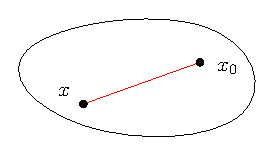
\includegraphics[width=0.3\textwidth ]{images/insieme_stellato.eps}
\end{center}
Si può scrivere la differenza fra $f(x)$ e $f(x_0)$ sotto forma di integrale:\begin{align}
    &f(x)-f(x_0)=\int_0^1\frac{\partial}{\partial t}f(x_0+t(x-x_0))dt=\\
    &\sum_{j=1}^n(x^j-x_0^j)\int_0^1\frac{\partial f}{\partial x^j}(x_0+t(x-x_0))dt
\end{align}
Si definisce $g_j$ come segue\begin{equation}
    g_j(x)=\int_0^1\frac{\partial f}{\partial x^j}(x_0+t(x-x_0))dt
\end{equation}
chiaramente \begin{align}
     &g_j(x_0)=\int_0^1\frac{\partial f}{\partial x_0^j}(x_0+t(x_0-x_0))dt=\\
     &\int_0^1\frac{\partial f}{\partial x_0^j}(x_0)dt=
     \frac{\partial f}{\partial x_0^j}(x_0)\int_0^1dt
     =\frac{\partial f}{\partial x^j}(x_0)
\end{align}
allora \begin{align}
    &f(x)-f(x_0)=\sum_{j=1}^n(x^j-x_0^j)g_j(x)\implies\\
    &f(x)=f(x_0)+\sum_{j=1}^n(x^j-x_0^j)g_j(x).
\end{align}
$g_j(x)$ sono di classe $C^\infty$ in $U$ quindi sono contenute nei germi $g_j\in C_{x_0}^\infty$.\hfill$\blacksquare$
\begin{osservazione}
    Tale lemma è valido esclusivamente per funzioni di classe $C^\infty$.
\end{osservazione}
Si vuole dimostrare ora che $ \dim X=n\implies\dim T_pX=n$, si dimostra prima un caso pià semplice in cui la varietà $X$ è un'aperto di $\R^n$, si sfrutta poi il fatto che localmente ogni varietà è identificata tramite una carta locale da un'aperto di $\R^n$.
\begin{proposizione}La proposizione è divisa in due punti.\bigskip

\noindent\boxedMath{1} Sia $U\subset\R^n$ un'aperto, sia $x_0\in U$, si consideri la funzione\begin{align}
        &\iota :\R^n\rightarrow T_{x_0}U\\
        &(a^1\dots,a^n)=v\longmapsto \iota(v)=\sum_{j=1}^na^j\frac{\partial}{\partial x^j}\hphantom{.}_{|x_0}
    \end{align}
    $\iota(v)$ non è altro che la derivata direzionale nella direzione specificata da $v$. $\iota$ è un'isomorfismo di spazi vettoriali.\bigskip

    \noindent\boxedMath{2} Sia $X$ una $n$-varietà, e sia $p\in X$. Lo spazio tangente $T_pX$ è uno spazio vettoriale di dimensione $n$. Se $\varphi=(x^1\dots,x^n)$ è una carta locale in $p$, allora\begin{equation}
        \Big\{\frac{\partial}{\partial x^1}\hphantom{.}_{|p},
        \frac{\partial}{\partial x^2}\hphantom{.}_{|p},\dots
        \frac{\partial}{\partial x^n}\hphantom{.}_{|p}\Big\}
    \end{equation} 
    è una base per $T_pX$.
\end{proposizione}
\textit{Dimostrazione}: Si dimostrano separatamente i due punti.

\noindent\boxedMath{1}Si comincia col dimostrare che $\iota$ è un'isomorfismo, per definizione è chiaramente lineare, bisogna dimostrare che è biettiva. Sia $v=(a^1\dots, a^n)\ne 0$ un vettore, per qualche $1\le h\le n$, si ha $a^h\ne 0$. Si consideri l'immagine di $\iota$ su $v$:\begin{equation}
    \iota(v)=\sum_{j=1}^na^j\frac{\partial}{\partial x^j}\hphantom{.}_{|x_0}
\end{equation}
si deve dimostrare che $\iota(v)$ non è la derivazione nulla. Bisogna trovare una funzione tale per cui, applicando tale derivazione su questa funzione non si trova 0. Si consideri la funzione $\mathbf x:\R^n\rightarrow\R$ definita in tal modo \begin{equation}\label{eq:proiezione}
    \mathbf x^h(q^1\dots,q^n)=q^h
\end{equation}
ossia la funzione che ad ogni vettore associa la $h$-esima coordinata, si ha \begin{equation}
    \iota(v)(\mathbf x^h)=\sum_{j=1}^na^j\frac{\partial \mathbf x^h}{\partial x^j}\hphantom{.}_{|x_0}=\sum_{j=1}^{h-1}a^j\cdot 0+
    a^h
    +
    \sum_{j=h+1}^{n}a^j\cdot 0=a^h\ne 0
\end{equation}
quindi $\iota(v)$ non è la derivazione nulla, $\iota$ è quindi iniettiva. Bisogna ora dimostrare la suriettività di $\iota$, sia $D\in T_{x_0}U$ una qualunque derivazione. Bisogna trovare $v$ tale che $D=\iota(v)$.

Sia $ x^j\in C_{x_0}^\infty$ una funzione definita come in \eqref{eq:proiezione}, si pone $D( x^j)=a^j \in\R$. Si costruisce un vettore\begin{equation}
    v=(a^1,a^2\dots a^n)=(D( x^1)\dots,D( x^n))
\end{equation}
Si vuole dimostrare che $D=\iota(v)$, ossia, si vuole mostrare che $D(f)=\iota(v)(f)$ per ogni $f\in C_{x_0}^\infty$. Si utilizza il Lemma \ref{lemma:funzioni_g}:\begin{align}
    &D(f)=D[f(x_0)+\sum_{j=1}^n(x^j-x_0^j)g_j(x)]=\\
    &D(f(x_0))+\sum_{j=1}^nD[(x^j-x_0^j)g_j(x)]
\end{align}
$D(f(x_0))$ è 0 dato che $f(x_0)$ è una costante
\begin{align}
    &D(f(x_0))+\sum_{j=1}^nD[(x^j-x_0^j)g_j(x)]=\\
    &\sum_{j=1}^nD[(x^j-x_0^j)g_j(x)]
\end{align}
essendo che $D$ è una derivazione, si applica la regola di Leibniz
\begin{align}
    &\sum_{j=1}^n[D(x^j-x_0^j)g_j(x_0)+((x^j(x_0)-x_0^j))D(g_j)]
\end{align}
per definizione $x^j(x_0)=x_0^j$ quindi 
\begin{align}
    &\sum_{j=1}^n[D(x^j-x_0^j)g_j(x_0)+((x^j(x_0)-x_0^j))D(g_j)]=\\
    &\sum_{j=1}^n[D(x^j-x_0^j)g_j(x_0)+((x^j_0-x_0^j))D(g_j)]=\\
     &\sum_{j=1}^n D(x^j-x_0^j)g_j(x_0)
\end{align}
si sfrutta nuovamente l'additività di $D$
\begin{align}
     &\sum_{j=1}^n D(x^j-x_0^j)g_j(x_0)=\\
     &\sum_{j=1}^n [D(x^j)-D(x_0^j)]g_j(x_0)=\\
      &\sum_{j=1}^n D(x^j)g_j(x_0)
\end{align}
per definizione $D(x^j)=a^j$
\begin{align}
      &\sum_{j=1}^n D(x^j)g_j(x_0)=\\
      &\sum_{j=1}^n a^jg_j(x_0)
\end{align}
per il lemma, la funzione $g_j$ in $x_0$ assume lo stesso valore della derivata parziale di $f$ rispetto $x^j$\begin{align}
     &\sum_{j=1}^n a^jg_j(x_0)=\\
      &\sum_{j=1}^n a^j\frac{\partial f}{\partial x^j}(x_0)=\iota(v)(f).
\end{align}
Si è dimostrato che $D=\iota(v)$, $\iota$ è un'isomorfismo di spazi vettoriali, $T_{x_0}U$ ha la stessa dimensione di $U\subset\R^n$.\bigskip

\noindent\boxedMath{2} Bisogna mostrare che lo stesso risultato si estende ad ogni varietà. Sia $X$ una varietà con $p\in X$, sia $(U,\varphi)$ una carta locale con $p\in U$. È banale che $\varphi$ sia un diffeomorfismo di varietà, sappiamo essere un omeomorfismo fra $X$ e $\R^n$\begin{equation}
    X\supset U \longrightarrow V=\varphi(U)\subset\R^n
\end{equation}
se l'espressione locale di $\varphi$ è un diffeomorfismo fra aperti di $\R^n$ allora anche $\varphi$ lo è, ma la rappresentazione locale di $\varphi$ è la composizione fra $\varphi$ e $\varphi^{-1}$ (è l'identità in $V$).
\begin{center}
\begin{tikzpicture}
    \matrix (m) [matrix of math nodes, row sep=3em, column sep=3em, minimum width=2em]
    {
        X \supset U & V \subset \mathbb{R}^n \\
        \mathbb{R}^n \supset \varphi(U) = V & V \subset \mathbb{R}^n \\
    };
    \path[->] (m-1-1) edge node[above] {$\varphi$} (m-1-2);
    \path[->] (m-2-1) edge node[above] {$\widetilde{\varphi}$} (m-2-2);
    \path[->] (m-1-1) edge node[left] {$\varphi$} (m-2-1); % Adjusted position to 'left'
    \path[->] (m-1-2) edge node[right] {Id} (m-2-2);
\end{tikzpicture}
\end{center}
L'identità è ovviamente un diffeomorfismo. Si consideri il differenziale di $\varphi$ in $p$\begin{equation}
    d\varphi_p:T_pU=T_pX\longrightarrow T_{\varphi(p)}\varphi(U)
\end{equation}
Ma $T_{\varphi(p)}\varphi(U)$ è isomorfo ad $\R^n$ (per il punto 1 della dimostrazione). Per le proprietà del differenziale, se la funzione fra varietà $\varphi$ è un diffeomorfismo, il differenziale $d\varphi_p$ è un'isomorfismo, ma questo allora è isomorfo ad $\R^n$, allora la dimensione di $T_pX$ è $n$. Un'isomorfismo mappa i vettori di una base nell'altra, i vettori \begin{equation}
        \Big\{\frac{\partial}{\partial x^1}\hphantom{.}_{|p},
        \frac{\partial}{\partial x^2}\hphantom{.}_{|p},\dots
        \frac{\partial}{\partial x^n}\hphantom{.}_{|p}\Big\}
    \end{equation} 
Sono le immagini tramite $d\varphi_p^{-1}$ dei vettori della base canonica di $\R^n$, sono quindi una base per $T_pX$.\hfill$\blacksquare$\bigskip


\noindent In conclusione, lo spazio tangente in un punto di una varietà $n$-dimensionale è isomorfo ad $\R^n$.
\end{document}

